% This must be in the first 5 lines to tell arXiv to use pdfLaTeX, which is strongly recommended.
\pdfoutput=1
% In particular, the hyperref package requires pdfLaTeX in order to break URLs across lines.

\documentclass[11pt]{article}

% Remove the "review" option to generate the final version.
% \usepackage[review]{ACL2023}
\usepackage{ACL2023}

% Standard package includes
\usepackage{times}
\usepackage{latexsym}
\usepackage{fontawesome}
\usepackage{amsmath}
\usepackage{bm}
\usepackage{amsfonts}
\usepackage{amssymb}
\usepackage{booktabs}
\usepackage{subcaption}
\usepackage{caption}
\usepackage{graphicx}
\usepackage{multirow}
% For proper rendering and hyphenation of words containing Latin characters (including in bib files)
\usepackage[T1]{fontenc}
% For Vietnamese characters
% \usepackage[T5]{fontenc}
% See https://www.latex-project.org/help/documentation/encguide.pdf for other character sets

% This assumes your files are encoded as UTF8
\usepackage[utf8]{inputenc}

% This is not strictly necessary, and may be commented out.
% However, it will improve the layout of the manuscript,
% and will typically save some space.
\usepackage{microtype}

% This is also not strictly necessary, and may be commented out.
% However, it will improve the aesthetics of text in
% the typewriter font.
\usepackage{inconsolata}
\usepackage{makecell}
\usepackage{xcolor}
\usepackage{todonotes}
% If the title and author information does not fit in the area allocated, uncomment the following
%
%\setlength\titlebox{<dim>}
%
% and set <dim> to something 5cm or larger.

\newcommand\blfootnote[1]{%
  \begingroup
  \renewcommand\thefootnote{}\footnote{#1}%
  \addtocounter{footnote}{-1}%
  \endgroup
}



\title{Recall, Expand and Multi-Candidate Cross-Encode: \\
Fast and Accurate Ultra-Fine Entity Typing}


% Author information can be set in various styles:
% For several authors from the same institution:
\author{
    \textbf{Chengyue Jiang$^\Diamond$$^\ddagger$},
    \textbf{Wenyang Hui$^\Diamond$$^\ddagger$},
    \textbf{Yong Jiang},
    \textbf{Xiaobin Wang},
    \textbf{Pengjun Xie},
    \textbf{Kewei Tu$^\ddagger$}\thanks{$~~$ Kewei Tu is the corresponding author.} \\
    $^\ddagger$ School of Information Science and Technology, ShanghaiTech University \\
    Shanghai Engineering Research Center of Intelligent Vision and Imaging \\
    \texttt{\{jiangchy,huiwy,tukw\}@shanghaitech,edu.cn;} \\
    \texttt{\{jiangyong.ml,xpjandy\}@gmail.com;} \\
    \texttt{czwangxiaobin@foxmail.com;}
}

\begin{document}
\maketitle

\blfootnote{$^\Diamond$ Equal Contribution.}
\newcommand{\code}{\url{http://github.com/modelscope/AdaSeq/tree/master/examples/MCCE}}
\newcommand{\name}{{MCCE}}

	
\begin{abstract}

Continuous Integration (CI) is a software development practice that builds and tests software frequently (e.g., at every push). One main motivator to adopt CI is the potential to deliver software functionalities more quickly than not using CI. However, there is little empirical evidence to support that CI helps projects deliver software functionalities more quickly. Through the analysis of 162,653 pull requests (PRs) of 87 GitHub projects, we empirically study whether adopting a CI service (\textsc{TravisCI}) can quicken the time to deliver merged PRs. 
We complement our quantitative study by analyzing 450 survey responses from participants of 73 software projects.
Our results reveal that adopting a CI service may not necessarily quicken the delivery of merge PRs. Instead, the pivotal benefit of a CI service is to improve the decision making on PR submissions, without compromising the quality or overloading the project's reviewers and maintainers. The automation provided by CI and the boost in developers' confidence are key advantages of adopting a CI service. Furthermore, open-source projects planning to attract and retain developers should consider the use of a CI service in their project, since CI is perceived to lower the contribution barrier while making contributors feel more confident and engaged in the project.
		
\keywords{Continuous Integration \and Pull Request \and Delivery Time \and Code Review}
 
\end{abstract}

\section{Introduction}
\label{sec:introduction}
Before the early 1960s, it was believed that $CP$ is a good symmetry of nature. As Landau pointed out, that would make it impossible for particles to have electric dipole moments (EDMs) along their spin axis \cite{landau1957conservation}. The detection of such an EDM would thus provide clear evidence of $CP$-violation (CPV).  \blfootnote{*Present address: JILA, National Institute of Standards and Technology and University of
Colorado, and Department of Physics, Boulder, Colorado 80309, USA}

While most processes preserve $CP$, certain weak interactions violate it as observed in $K$-, $B$-, and $D$-meson decays \cite{christenson1964evidence, PDG18}. The flavor-changing part of the Standard Model (SM) quark sector includes a CPV phase in the CKM quark-mixing matrix \cite{peccei1995}. This so-called Kobayashi-Maskawa mechanism introduces the third quark generation to explain the CPV \cite{kobayashi1973cp}. The CKM phase has been the only source of observed CPV so far~\cite{PDG18}.

A major motivation for CPV searches comes from the baryon asymmetry of the universe (BAU). Compared to the current baryon density $n_{\text{B}}$, the antibaryon density $n_{\overline{\text{B}}}$ is very small; the reported upper bounds for the antimatter-to-matter number ratio range from $10^{-15}$ to $10^{-6}$ \cite{canetti2012matter}. To date, no mechanism has been experimentally verified that can explain the BAU. In a 1967 paper, Sakharov argued that CPV is necessary to explain the BAU \cite{sakharov1991violation} if the initial conditions of the universe were $C$-symmetric. The existing CPV in the CKM matrix is not enough to explain the extent of the BAU \cite{pospelov2005electric}. Thus new sources of CPV are required to explain the BAU.

No flavor-neutral CPV signal has been observed yet. However, many mechanisms can lead to such phenomena. For example, the QCD Lagrangian can, in principle, include an effective CPV term, proportional to the parameter $\bar{\theta}$~\cite{pospelov1999theta}:
\begin{equation}
	\mathcal{L} = \bar{\theta}\frac{g^2}{32\pi^2}G^a_{\mu\nu}\widetilde{G}^a_{\mu\nu},
\end{equation}
where $G^a$ is the gluon field tensor, $g$ is the strong coupling constant, and $\bar{\theta}$ is dimensionless. Experimental limits from experiments searching for CPV in neutral $^{199}$Hg atoms \cite{graner2016reduced} and ultracold neutrons \cite{baker2006improved, abel2020measurement} suggests that the strength of this term relative to the usual strong interaction is $\left|\bar{\theta}\right|<9\cdot10^{-11}$. The unexplained smallness of $\bar{\theta}$ is known as the strong $CP$ problem. One proposed solution to the strong $CP$ problem is the so called Peccei-Quinn mechanism, with an accompanying elementary scalar particle: the axion \cite{PhysRevLett.38.1440}. The axion would naturally lead to $\bar{\theta}\approx 0$, and is an attractive candidate for dark matter~\cite{PRESKILL1983127,PhysRevLett.50.925,PhysRevLett.124.101303}. (A review of experimental searches for the axion is given in \cite{graham2015experimental}.)

New hadronic $CP$-violating interactions from the QCD sector, or from physics beyond the SM, can lead to an effective charge asymmetry along the spin of a particle. Such charge asymmetries include EDMs and, for finite size particles such as nuclei, Schiff moments \cite{schiff1963measurability}. In the Standard Model, EDMs and nuclear Schiff moments (NSMs) are induced by the CKM phase, but are strongly suppressed: an EDM cannot appear below the three-loop level for quarks, or four-loop for leptons \cite{pospelov1991electric}. The CKM phase can produce a proton or neutron EDM no larger than $10^{-32}\,e\,$cm. Proposed extensions to the SM carry new CPV phases, which may manifest as EDMs or NSMs larger than expected based on the Standard Model. The search for an EDM or NSM thus constitutes a nearly background-free signal for new physics. In fact, the background expected from the Standard Model would only become apparent when probing effects beyond the energy scale of $\sim\!10^{5}\,$TeV \cite{pospelov2005electric}.

At present, searches for EDMs and related phenomena give the most sensitive constraints on flavor-neutral CPV effects beyond the SM. However, these searches are subject to the following limitation. According to the Schiff theorem, the interaction energy of nonrelativistic point-charged electric dipoles, bound in a neutral system but subject to an arbitrary external electrostatic potential, has no term linear in the CPV charge distribution \cite{schiff1963measurability}. Physically, the system rearranges itself so as to screen the external field completely \cite{safronova2018search}. Thus, a $CP$-violating moment of a charged constituent in a bound system cannot be detected without some mechanism to bypass Schiff's theorem. Two such mechanisms are relativistic constituent motion and finite constituent size. 

A nucleus in an atom or molecule is nonrelativistic, but has an extended size. This finite size can lead to a residual electromagnetic moment, the Schiff moment $\vec S$, that gives rise to a $CP$-violating interaction. In heavy diamagnetic atoms and diatomic molecules such as TlF, this finite-size effect gives the dominant contribution to CPV signals. Since the nuclear spin $\vec{I}$ is the only preferred direction in a nucleus, $\vec S$ has to lie parallel to this axis, i.e., $\vec{S} = S\vec{I}/I$. This quantum Schiff moment has the symmetries of $\vec{I}$: it changes sign under time reversal ($T$) but not under parity ($P$). By contrast, the classical Schiff moment is a static charge distribution that is unchanged under $T$ but changes sign under $P$. Hence, a nonzero value of $S$ means that both $T$ and $P$ symmetries are violated.
On the assumption that $CPT$ is a good symmetry, a nonzero value of $\vec S$ thus is also a signature of CPV.

The Schiff moment corresponds to a charge displacement that is similar to an EDM in its asymmetric distribution along the spin axis. It is equivalent to a charge density on the nuclear surface proportional to $\cos{\theta}$, where $\theta$ is the angle from $\vec{I}$; this surface charge distribution produces a uniform electric field inside the nucleus \cite{GingesFlambaum2004}. The magnitude $S$ of the NSM scales with the atomic mass $A$ as $S\propto A^{2/3}$ \cite{khriplovich1997}.

The value of $S$ can be related to more fundamental $CP$-violating parameters, including CPV $\pi$ meson--nucleon interaction constants $\bar{g}_{0},\,\bar{g}_1,$ and $\bar{g}_2$; the $\bar{\theta}$ QCD parameter; quark chromo-EDMs $\widetilde{d}_\text{d}$ and $\widetilde{d}_\text{u}$; and the neutron and proton EDMs, $d_\text{n}$ and $d_\text{p}$.  For example, the NSM of the $^{205}\mathrm{Tl}$ nucleus\footnote{The $^{205}\mathrm{Tl}$ nucleus has closed neutron shells; hence its NSM has negligible contribution from $d_\text{n}$.}  can be written as \cite{PhysRevA.101.042504,PhysRevA.101.042501}:
\begin{equation} 
    \label{eq:schiff_contributions}
        \begin{split}
            S\left(^{205}\mathrm{Tl}\right) & \approx \left(0.13g\bar{g}_0 - 0.004g\bar{g}_1 - 0.27 g \bar{g}_2\right) \,e\,\mathrm{fm}^3; \\
            S\left(^{205}\mathrm{Tl}\right) & \approx 0.027 \bar{\theta}\ e\,\mathrm{fm}^3; \\
            S\left(^{205}\mathrm{Tl}\right) & \approx \left(12\widetilde{d}_\text{d}+9\widetilde{d}_\text{u}\right) e\,\mathrm{fm}^2; \\
            S\left(^{205}\mathrm{Tl}\right) & \approx 0.4\,d_\text{p} \,\mathrm{fm}^2.
    \end{split}
\end{equation}
If detected, a nonzero $S\left(^{205}\mathrm{Tl}\right)$ would provide evidence for a nonzero value of one or more of these fundamental CPV parameters.

Energy shifts associated with a NSM can be greatly enhanced in polar molecules, where there is another intrinsic direction in addition to the nuclear spin: the internuclear axis $\hat{\vec{n}}$. In TlF,  we define $\hat{\vec{n}}$ as pointing from F to Tl, associated with the internal molecular dipole moment and a corresponding strong intramolecular gradient of the electron density.  For nuclei inside a molecule, the NSM (and other $CP$-violating effects \cite{khriplovich1997}) interacts with this density gradient, giving rise to an effective CPV Hamiltonian of the form \cite{PhysRevA.101.042504}
\begin{equation}\label{eq:Hamiltonian_effective_interaction}
    \mathcal{H}_\text{CPV}= W_S S\,\frac{\vec{I}}{I} \cdot \hat{\vec{n}}.
\end{equation}
Here, $W_S$ is the proportionality constant between $S$ and the CPV contribution to the molecular energy, for a fully polarized molecule. Its value is determined by the properties of the electronic wavefunctions, which can be calculated from first principles \cite{PhysRevA.101.042504, doi:10.1002/qua.20418, PhysRevLett.88.073001, doi:10.1080/00268976.2020.1767814}. The magnitude of $W_S$ grows rapidly with atomic number $Z$ of the nucleus, as $W_S\propto Z^2$ \cite{khriplovich1991parity}.

Without an external electric field $\Evec$, the interaction of Eq.~\ref{eq:Hamiltonian_effective_interaction} fails to produce a first-order effect in any given energy eigenstate. This is because the rotation of the molecule averages $\hat{\vec n}$ to zero, and the expectation value $\langle\mathcal{H}_\text{CPV}\rangle$ vanishes \cite{cho1989tenfold, cho1991search}. However, when an external field is applied, the molecule becomes polarized and both
%which destroys the inversion symmetry; then
$\hat{\vec{n}}$ and $\mathcal{H}_\text{CPV}$  acquire non-zero expectation values, with $\langle\hat{\vec n}\rangle \parallel \Evec$. We define the degree of electrical polarization $\mathcal{P} \equiv \langle \hat{\vec{n}}\cdot\hat{\Evec} \rangle$, (where $\hat{\Evec} = \Evec/\Esca$), so that $-1\leq\mathcal{P}\leq1$. 
%Here $\hat{z}$ is defined to be the axis along which the external electric field is applied. 
Hence, energy shifts due to CPV are given by  $\langle\mathcal{H}_\text{CPV}\rangle = W_S S \mathcal{P} \hat{\Evec} \cdot \frac{\vec{I}}{I}$.

\begin{figure}
    \centering
    \def\svgwidth{0.5\textwidth}
    \input{figs/svg/edm_levels.pdf_tex}
% 	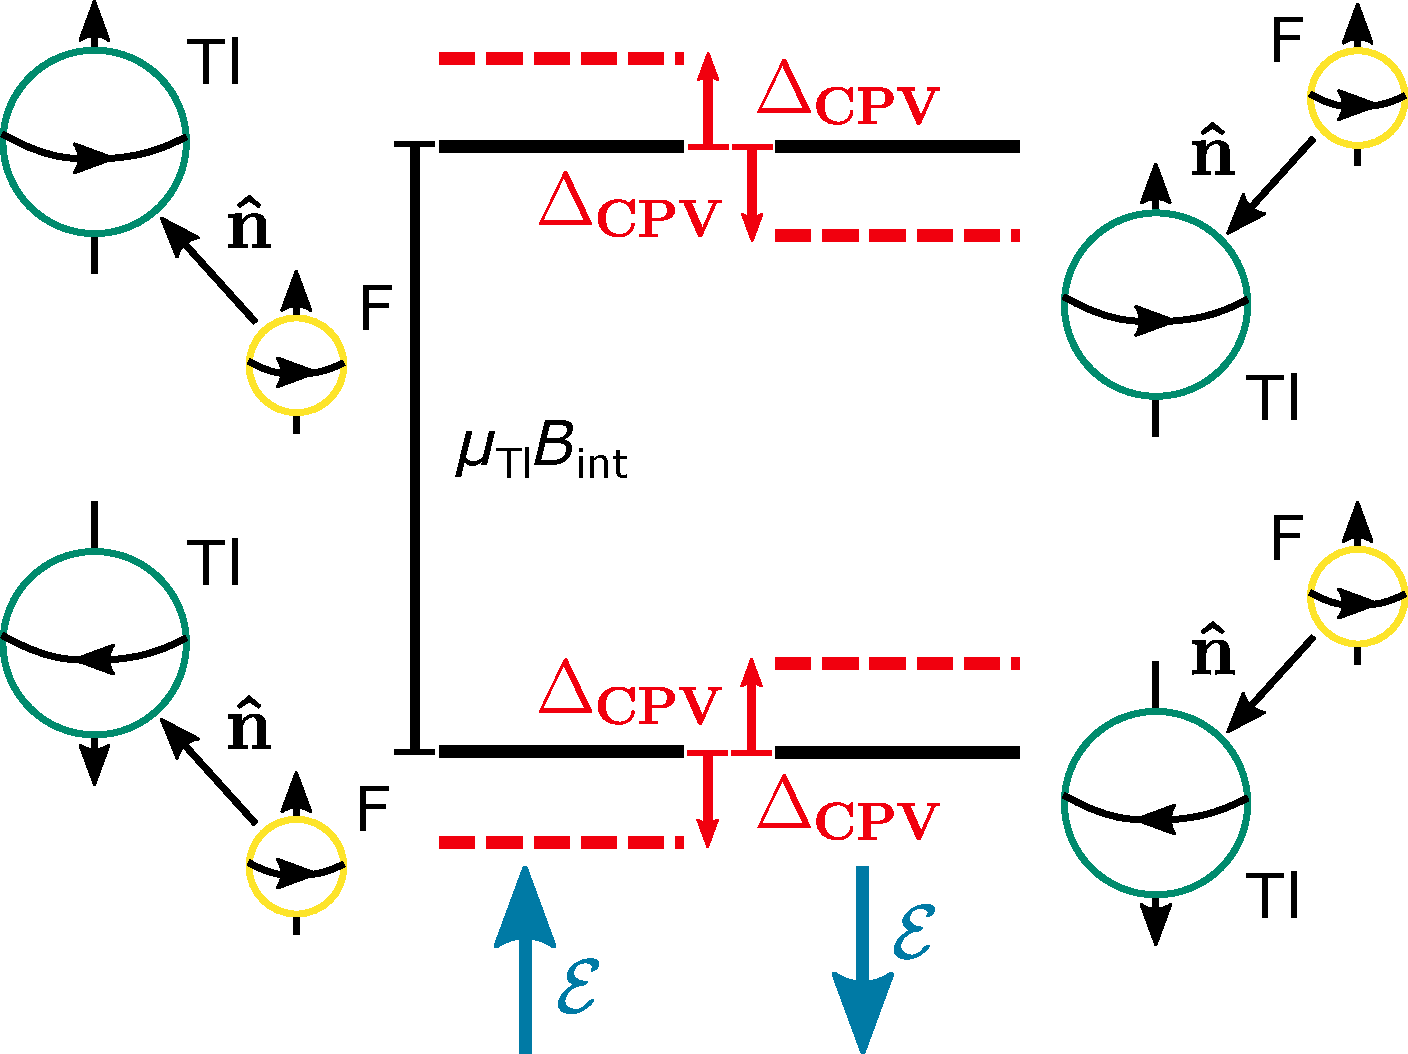
\includegraphics[width=0.48\textwidth,unit=1mm]{figs/svg/edm_levels_pdf_version.pdf}
	\caption{T-violating energy shift $\Delta_{\rm CPV} = W_SS\,\mathcal{P}$ as a result of a nonzero NSM $S$ given by the effective interaction $\mathcal{H}_\text{CPV}= W_S S\vec{I}\cdot \hat{\vec{n}}/I$ (Eq.~\ref{eq:Hamiltonian_effective_interaction}), shown for opposite orientations of the applied field $\Evec$. Here $\mu_1$ is the Tl magnetic moment and $B_1^\mathrm{int}$ is the effective internal magnetic field at the Tl nucleus due to the spin-rotation interaction.
	}
	\label{fig:edm_shift}
\end{figure}

Polar molecules can be polarized readily in laboratory-scale fields owing to their small rotational level separation ($\sim\!10^{-4}\eV$), giving them near-maximal energy shifts induced by a given Schiff moment. Thus, Sandars \cite{sandars1967measurability} suggested a molecular-beam resonance experiment could be used to probe the existence of the proton EDM, if the molecule has a heavy atom with an unpaired proton in the nucleus, such as $^{205}\mathrm{Tl}$. The value of $S$ is determined by measuring energy splittings between spin-up and -down states relative to $\left\langle \hat{\vec{n}}\right\rangle$ (which is parallel to the applied electric field $\bm{\mathcal{E}}$). This splitting will increase or decrease as $\bm{\mathcal{E}}$ (and hence $\left\langle \hat{\vec{n}}\right\rangle$) reverses, due to the interaction in Eq.~\ref{eq:Hamiltonian_effective_interaction}. The difference in level splittings is proportional to the electric polarization $\mathcal{P}$, the interaction strength $W_S$, and $S$ (Fig. \ref{fig:edm_shift}).

\CENTREX\ uses a cold beam of thallium fluoride (TlF) to measure nuclear $T$-violation due to the NSM of the $^{205}$Tl nucleus. It is a suitable system to look for $P$- and $T$-violating interactions for a number of reasons: a molecular beam of thallium fluoride can be readily obtained; many of the molecular states and transitions are known experimentally; the species is a polar diatomic molecule, enhancing the electron density gradient at the site of the nuclei (and hence $W_S$). As the thallium nucleus is heavy $\left(A=205,\,Z=81\right)$ and the NSM-induced energy shift scales $\propto A^{2/3}Z^2$, the observable effect of the Tl Schiff moment is correspondingly large \cite{sandars1967measurability, wilkening1984search}. Since the Tl nucleus contains an unpaired proton,
%the different linear combinations of underlying CPV parameters means
\CENTREX\ will be primarily sensitive to proton EDM effects, as opposed to other leading experiments which are more sensitive to the
%effects associated with neutron spin such as
neutron EDM \cite{graner2016reduced}. TlF is not very sensitive to the electron EDM due to its zero total electron spin \cite{kozlov1995parity}. 

The current best constraint on $T$-violating interactions associated with $S\left(^{205}\mathrm{Tl}\right)$ was found by Cho, Sangster and Hinds in 1991 \cite{cho1989tenfold, cho1991search}, who measured a NSM-induced frequency shift of $\Delta E = 2\Delta_{\rm CPV} = \left(1.4\pm 2.4\right)\times 10^{-4}$~Hz, consistent with zero.\footnote{Throughout, we express both frequencies and energies in linear frequency units (Hz), and all angular momentum operators are treated as dimensionless.} 
Using the effective interaction $\mathcal{H}_\text{CPV}$, the shift in the energy splitting between states with Tl spin up versus spin down, relative to the quantization axis, can be interpreted as
\begin{equation}
    \Delta E= 2 \Delta_{\rm CPV} = 2 W_S\,S\, \textrm{sgn}(\Esca) \,\mathcal{P},
    \label{eq:frequency_shift_due_to_NSM}
\end{equation}
where $W_S = 40539\,$a.u.,
polarization $\mathcal{P} = \langle\hat{\vec{n}} \cdot \hat{\Evec}\rangle = 0.547$, and the sign of $\Esca$ refers to the direction of $\Evec$ relative to a fixed quantizing axis $\hat{z}$.  This determines the Schiff moment \cite{PhysRevA.101.042501, PhysRevLett.88.073001}
\begin{equation}
    S\left(^{205}\mathrm{Tl}\right) = \left(3.6\pm 6.1\right)\times 10^{-11}\,e\,\mathrm{fm}^3.
\end{equation}
With Eq.~\ref{eq:schiff_contributions}, the following limits can be placed:
\begin{equation}
    \label{eq:prev_best_lims}
    \begin{split}
        \bar{\theta} & = \left(1.3 \pm 2.3\right)\ee{-9}, \\
        12\bar{d}_d+9\bar{d}_u & = \left(3.6\pm 6.1\right)\ee{-24}\,\mathrm{cm}, \\
        d_p          & = \left(0.9 \pm 1.5\right)\ee{-23}\,e\,\mathrm{cm},\\
        0.13g\bar{g}_0 - 0.004g\bar{g}_1-0.27g\bar{g}_2 & = \left(3.6 \pm 6.1\right)\ee{-11}.
    \end{split}
\end{equation}
\CENTREX\ aims to improve on these limits by using a cryogenic molecular beam source to achieve a cold beam with higher intensity and lower velocity spread compared to the jet source used in the previous work. Rotational cooling will be performed with optical and microwave pumping, collapsing much of the initial Boltzmann distribution into one state, greatly enhancing the number of molecules accessible for measurement. Finally, optical cycling will be used to assist state readout, resulting in near-unity detection efficiency. Fluorescence detection, compared to the hot-wire techniques used previously, allows for background-free detection if scattered light is well controlled.

\subsection{Thallium Fluoride}
\label{sec:tlf_theory}

\begin{figure}
	    % for axis breaks
    \usetikzlibrary{decorations.markings}
    \def\MarkLt{4pt}
    \def\MarkSep{2pt}
    \tikzset{
      TwoMarks/.style={
        postaction={decorate,
          decoration={
            markings,
            mark=at position #1 with
              {
                  \begin{scope}[xslant=0.2]
                  \draw[line width=\MarkSep,white,-] (0pt,-\MarkLt) -- (0pt,\MarkLt) ;
                  \draw[-] (-0.5*\MarkSep,-\MarkLt) -- (-0.5*\MarkSep,\MarkLt) ;
                  \draw[-] (0.5*\MarkSep,-\MarkLt) -- (0.5*\MarkSep,\MarkLt) ;
                  \end{scope}
              }
           }
        }
      },
      TwoMarks/.default={0.5},
    }

\begin{tikzpicture}[scale=5]

   % length of energy level diagram lines
   \def\len{.05}

   % x-position and length and x-offset of the y-axis labels
   \def\pos{-18}
   \def\lenmark{.025}
   \def\xoffset{.18}

   % x coordinates for m = -2, ... 2
   \def\xa{-4.5*\len}
   \def\xb{-2.5*\len}
   \def\xc{-0.5*\len}
   \def\xd{+1.5*\len}
   \def\xe{+3.5*\len}
   \def\xf{-6.5*\len}
   \def\xg{+5.5*\len}

   % y offset for J = 1, 2
   \def\yA{.6}
   \def\yB{\yA+.7}

   % axis
   \draw[->,TwoMarks=0.2,TwoMarks=0.6] (\xf-\len-\xoffset, -.1)
      -- (\xf-\len-\xoffset,\yB+.25) node[above, xshift = -20] {$E$ [kHz]};

   % brace position
   \def\bracePos{\xg+3*\len}

    
   % J=0 labels
   \draw [decorate,decoration={brace,amplitude=5pt,mirror,raise=4pt},yshift=0pt]
      (\bracePos,-.08) -- node (midJ0) {} (\bracePos,.08) node [black,midway,anchor=west,xshift=25] (nodeJ0) {$0$};
   \draw (\xf-\len-0.5*\lenmark-\xoffset, -.003325) node[anchor=east,below,xshift=\pos]
      {-3.325} -- (\xf-\len+0.5*\lenmark-\xoffset,-.003325) node[right,below,xshift=-\pos] {$1$};
   \draw (\xf-\len-0.5*\lenmark-\xoffset, .009975) node[anchor=east,above,xshift=\pos]
      {9.975} -- (\xf-\len+0.5*\lenmark-\xoffset,.009975) node[right,above,xshift=-\pos] {$0$};

   % J=0 lines
   \draw (\xc, -0.003325) -- (\xc+\len, -0.003325);
   \draw (\xb, -0.003325) -- (\xb+\len, -0.003325);
   \draw (\xd, -0.003325) -- (\xd+\len, -0.003325);
   \draw (\xc, 0.009975) -- (\xc+\len, 0.009975);

   % J=1 labels
   \draw [decorate,decoration={brace,amplitude=10pt,mirror,raise=4pt},yshift=0pt]
      (\bracePos,\yA-.2) -- node (midJ1) {} (\bracePos,\yA+.1) node [black,midway,anchor=west,xshift=25] (nodeJ1) {$1$};
   \draw (\xf-\len-0.5*\lenmark-\xoffset, \yA-.143745) node[anchor=east,below,xshift=\pos] {-143.745} --
      (\xf-\len+0.5*\lenmark-\xoffset,\yA-.143745) node[right,below,xshift=-\pos] {$0$};
   \draw (\xf-\len-0.5*\lenmark-\xoffset, \yA-.121506) node[anchor=east,above,xshift=\pos] {-121.506} --
      (\xf-\len+0.5*\lenmark-\xoffset,\yA-.121506) node[right,above,xshift=-\pos] {$1$};
   \draw (\xf-\len-0.5*\lenmark-\xoffset, \yA+.054446) node[anchor=east,below,xshift=\pos] {54.446} --
      (\xf-\len+0.5*\lenmark-\xoffset,\yA+.054446) node[right,below,xshift=-\pos] {$1$};
   \draw (\xf-\len-0.5*\lenmark-\xoffset, \yA+.068985) node[anchor=east,above,xshift=\pos] {68.985} --
      (\xf-\len+0.5*\lenmark-\xoffset,\yA+.068985) node[right,above,xshift=-\pos] {$2$};

   % J=1 lines
   \draw (\xc, \yA-.143745) -- (\xc+\len, \yA-.143745);
   \draw (\xc, \yA-.121506) -- (\xc+\len, \yA-.121506);
   \draw (\xb, \yA-.121506) -- (\xb+\len, \yA-.121506);
   \draw (\xd, \yA-.121506) -- (\xd+\len, \yA-.121506);
   \draw (\xc, \yA+.054446) -- (\xc+\len, \yA+.054446);
   \draw (\xb, \yA+.054446) -- (\xb+\len, \yA+.054446);
   \draw (\xd, \yA+.054446) -- (\xd+\len, \yA+.054446);
   \draw (\xc, \yA+.068985) -- (\xc+\len, \yA+.068985);
   \draw (\xb, \yA+.068985) -- (\xb+\len, \yA+.068985);
   \draw (\xd, \yA+.068985) -- (\xd+\len, \yA+.068985);
   \draw (\xa, \yA+.068985) -- (\xa+\len, \yA+.068985);
   \draw (\xe, \yA+.068985) -- (\xe+\len, \yA+.068985);

   % J=2 labels
   \draw [decorate,decoration={brace,amplitude=10pt,mirror,raise=4pt},yshift=0pt]
      (\bracePos,\yB-.27) -- node (midJ2) {} (\bracePos,\yB+.18) node [black,midway,anchor=west,xshift=25] (nodeJ2) {$2$};
   \draw (\xf-\len-0.5*\lenmark-\xoffset, \yB-.217455)
   node[anchor=east,left,yshift=-5] {-217.455}
      -- (\xf-\len+0.5*\lenmark-\xoffset,\yB-.217455) node[right,below,xshift=-\pos] {$1$};
   \draw (\xf-\len-0.5*\lenmark-\xoffset, \yB-.172936)
   node[anchor=east,left,yshift=5] {-172.936}
      -- (\xf-\len+0.5*\lenmark-\xoffset,\yB-.172936) node[right,above,xshift=-\pos] {$2$};
   \draw (\xf-\len-0.5*\lenmark-\xoffset, \yB+.105876)
   node[anchor=east,left,yshift=-5] {105.876}
      -- (\xf-\len+0.5*\lenmark-\xoffset,\yB+.105876) node[right,below,xshift=-\pos] {$2$};
   \draw (\xf-\len-0.5*\lenmark-\xoffset, \yB+.141095)
   node[anchor=east,left,yshift=5] {141.095}
      -- (\xf-\len+0.5*\lenmark-\xoffset,\yB+.141095) node[right,above,xshift=-\pos] (J2F3label) {$3$};

   % J=2 lines
   \draw (\xc, \yB-.217455) -- (\xc+\len, \yB-.217455);
   \draw (\xb, \yB-.217455) -- (\xb+\len, \yB-.217455);
   \draw (\xd, \yB-.217455) -- (\xd+\len, \yB-.217455);
   \draw (\xc, \yB-.172936) -- (\xc+\len, \yB-.172936);
   \draw (\xb, \yB-.172936) -- (\xb+\len, \yB-.172936);
   \draw (\xd, \yB-.172936) -- (\xd+\len, \yB-.172936);
   \draw (\xa, \yB-.172936) -- (\xa+\len, \yB-.172936);
   \draw (\xe, \yB-.172936) -- (\xe+\len, \yB-.172936);
   \draw (\xc, \yB+.105876) -- (\xc+\len, \yB+.105876);
   \draw (\xb, \yB+.105876) -- (\xb+\len, \yB+.105876);
   \draw (\xd, \yB+.105876) -- (\xd+\len, \yB+.105876);
   \draw (\xa, \yB+.105876) -- (\xa+\len, \yB+.105876);
   \draw (\xe, \yB+.105876) -- (\xe+\len, \yB+.105876);
   \draw (\xc, \yB+.141095) -- (\xc+\len, \yB+.141095);
   \draw (\xb, \yB+.141095) -- (\xb+\len, \yB+.141095);
   \draw (\xd, \yB+.141095) -- (\xd+\len, \yB+.141095);
   \draw (\xa, \yB+.141095) -- (\xa+\len, \yB+.141095);
   \draw (\xe, \yB+.141095) -- (\xe+\len, \yB+.141095);
   \draw (\xf, \yB+.141095) -- (\xf+\len, \yB+.141095);
   \draw (\xg, \yB+.141095) -- (\xg+\len, \yB+.141095);

   % microwave energies
   \draw[Latex-Latex] (nodeJ0) -- node[above,sloped] {13.3 GHz} (nodeJ1);
   \draw[Latex-Latex] (nodeJ1) -- node[above,sloped] {26.7 GHz} (nodeJ2);

   % approximate F1 labels
   \def\FposX{-5}
   \def\FposY{15}
   \def\FposYY{22}
   \node[xshift=\FposX] at (midJ0) {\nicefrac{1}{2}};
   \node[xshift=\FposX,yshift=-\FposY] at (midJ1) {\nicefrac{1}{2}};
   \node[xshift=\FposX, yshift=\FposY] at (midJ1) {\nicefrac{3}{2}};
   \node[xshift=\FposX,yshift=-\FposYY] at (midJ2) {\nicefrac{3}{2}};
   \node[xshift=\FposX, yshift=\FposYY] at (midJ2) {\nicefrac{5}{2}};
   \node[xshift=\FposX, yshift=47] at (midJ2) (F1label) {$F_1$};
    
   \node at (F1label -| nodeJ2) {$J$};
   \node at (F1label -| J2F3label) {$F$};

\end{tikzpicture}

	\caption{Hyperfine structure in the lowest three rotational levels in the TlF ground state $X^1\Sigma^+$, with no applied fields. Rotational energies $hBJ(J+1)$ should be added to
	%are subtracted from
	the hyperfine energy shifts indicated on the axis. Note the $(2F+1)$-fold degeneracy of each state with total angular momentum $F$, corresponding to the quantum numbers $m_F=-F,\dots,0,\dots,F$.}
	\label{fig:level_diagram}

\end{figure}

The TlF molecule is described by its electronic, vibrational and rotational motion, plus the states of the Tl and F nuclear spins. \CENTREX\ makes use of states both in the vibronic ground state, $X ^1\Sigma^+\left(\nu=0\right)$, and in an electronically excited state, $B ^3\Pi_1\left(\nu=0\right)$.  In both cases, we describe the angular momentum couplings in a Hund's case (a) basis. We typically write energy eigenstates in terms of the basis states $\ket{\eta,J,F_1,F,m_F}$. Here, $\eta$ represents the vibronic quantum numbers; $J$ is the total angular momentum excluding the nuclear spins, $\vec{F}_1 = \vec{J}+\vec{I}_\mathrm{1}$, with $I_\mathrm{1}=1/2$ for $^{205}$Tl; $\vec{F} = \vec{F}_1+\vec{I}_\mathrm{2}$ is the total angular momentum, with $I_\mathrm{2}=1/2$ for $^{19}$F; and $m_F$ is its projection along a quantization axis in the lab frame. Field-free eigenstates are close to these basis states in the ground $X ^1\Sigma^+$ state.  In the $B ^3\Pi_1$ state, strong hyperfine interactions significantly mix states with different $J$ and $F_1$ values. Hence, we describe these eigenstates with the modified notation $\ket{\eta',\widetilde{J}' ,\widetilde{F}_1^\prime,F',m_F'}$, where $\widetilde{J}'$ and $\widetilde{F}_1^\prime$ correspond to the largest component in their basis-state decomposition; the primes indicate that the ket refers to the excited state $B ^3\Pi_1$.

Molecules in the beam are assumed to be in the vibronic ground state, since the beam temperature is much lower than the energy scales associated with the electronic and vibrational excitations. However, even at cryogenic temperatures, there is a Boltzmann distribution over many rotational and nuclear spin states. The dominant term in the energy of rotational/spin levels in the $X ^1\Sigma^+$ state is due to rotation; the mean energy of states with quantum number $J$ is $E_\mathrm{rot}=BJ(J+1)$, where $B\approx 6.67\GHz \approx 0.3\kelvin\,\kB$, where $\kB$ the Boltzmann constant.\footnote{In Ramsey et al.\ \cite{wilkening1984search}, the symbol $B$ denotes the rotational constant in equilibrium position, i.e., there $B\equiv B_\text{e}$. However, the effective $v=0$ rotational constant, $B_0$, is more relevant to \CENTREX. To first order in the Dunham expansion \cite{huber2013molecular}, $B_0=B_\text{e}-\alpha_\text{e}/2$. With $B_\text{e}$ and $\alpha_\text{e}$ from the NIST database \cite{afeefy2011nist}, we find $B_0$. We define the symbol $B\equiv B_0$; its value is shown in Table~\ref{tab:hyperfine_hamiltonian}.}

Hyperfine interactions split sublevels with different $F$ values ($F=J-1,J,J, J+1$, except $F=0,1$ only for $J=0$) in each rotational state. Thus, each rotational level has $4(2J+1)$ magnetic sublevels. %including nuclear spins.
Including rotation, spin-rotation and spin-spin interactions, plus interactions with external electric $(\Evec)$ and magnetic $(\Bvec)$ fields, the system is described by the effective Hamiltonian \cite{wilkening1984search}
\small
$\mathcal{H}_\text{TlF} = \mathcal{H}_\text{rot}+\mathcal{H}_\text{sr}+\mathcal H_\text{ss} + \mathcal H_\text{S}+\mathcal H_\text{Z}$, 
\normalsize
where
\begin{equation} 
    \label{eq:hyperfine_hamiltonian}
    \begin{split}
        \mathcal H_\text{rot} & = B \vec{J}^2 \\
        \mathcal H_\text{sr}&=c_1(\vec I_1\cdot\vec J)+c_2(\vec I_2\cdot\vec J), \\
        \mathcal H_\text{ss}&=c_3 T^2(\vec C)\cdot T^2(\vec I_1, \vec I_2)+c_4(\vec I_1\cdot\vec I_2), \\
        \mathcal H_\text{S}&=-\vec\mu_e\cdot\vec \Evec,\\
        \mathcal H_\text{Z}&=-\frac{\mu_J}{J}(\vec J\cdot\vec \Bvec)-\frac{\mu_1}{I_1}(\vec I_1\cdot\vec \Bvec)-\frac{\mu_2}{I_2}(\vec I_2\cdot\vec \Bvec).
    \end{split}
\end{equation}
Here, the first term in the spin-spin interaction ($\mathcal H_\text{ss}$) contains the scalar product of two rank-2 tensors: one constructed from the modified spherical harmonics $\vec C$, and one from $\vec{I}_1$ and $\vec{I}_2$ \cite{brown2003rotational}. (The matrix elements diagonal in $J$ of this term are given in \cite{wilkening1984search}.)  The hyperfine parameters $c_1,c_2,c_3,c_4$, rotational constant $B$, magnetic moments $\mu_J,\mu_1,\mu_2$, and molecule-frame electric dipole moment $\mu_e$ are all known from previous measurements; their values are given in  Table~\ref{tab:hyperfine_hamiltonian}. A level diagram of low-lying states in the absence of applied fields is shown in Fig.~\ref{fig:level_diagram}.

\begin{table}
    \small
    \setlength\extrarowheight{3pt}
    \rowcolors{2}{white}{gray!25}
	\centering
	\caption{Constants describing rotational, hyperfine, Zeeman, and Stark interactions in the effective TlF ground-state  Hamiltonian (Eq.~\ref{eq:hyperfine_hamiltonian}). All values taken from Ramsey et al.\ \cite{wilkening1984search}, except for $B$ (see Sec. \ref{sec:tlf_theory}).}
	\label{tab:hyperfine_hamiltonian}
	\begin{tabular}{r@{\hspace{5pt}}c@{\hspace{5pt}}l@{\hspace{5pt}}l | r@{\hspace{5pt}}c@{\hspace{5pt}}l@{\hspace{5pt}}l}
    	\toprule
		$B$ & = &           $6.66733$ &     GHz &       $\mu_e$ & = & $4.2282(8)$ &     Debye \\
		$\mu_J$ & = &       $35(15)$ &      Hz/G &      $c_1$ & = & $126.03(12)$ &    kHz \\
		$\mu_1^{205}$ & = & $1.2405(3)$ &   kHz/G &     $c_2$ & = & $17.89(15)$ &     kHz\\
		$\mu_1^{203}$ & = &  $1.2285(3)$ &   kHz/G &     $c_3$ & = & $0.70(3)$ &       kHz \\
		$\mu_2$ & = &      $2.00363(4)$ &  kHz/G  &    $c_4$ & = & $-13.30(72)$ &    kHz \\
		\bottomrule
	\end{tabular}
\end{table}

%%%%%%%%%%%%%%%%%%%%%%%%%%%%%%%%%%%%%%%%%%%%%%55%%%%%%%%%%%%%%%
In \CENTREX, lasers are tuned to $X^1\Sigma^+(\nu=0)\rightarrow B^3\Pi_1\left(\nu=0\right)$ transitions in order to manipulate and read out ground state hyperfine and rotational sublevels. Details of the $B ^3\Pi_1$ state structure are given in \cite{norrgard2017hyperfine,PhysRevA.101.042506}.  Here, only a few main features of the $B$ state substructure are important.  First, the $B$ state hyperfine splittings are very large ($\gtrsim 100\MHz$) compared to the natural linewidth of the transition ($\gamma_B \approx 1.6\MHz$), which is in turn much larger than the ground-state hyperfine splittings ($c_j \lesssim 100\kHz$). This means that hyperfine structure is fully resolved in the excited state, and entirely unresolved in the ground state. Hence, optical transitions in TlF drive a large manifold of ground-state hyperfine levels (with a given value of $J$) to a single hyperfine state with (nominal) quantum numbers $\tilde{J},\tilde{F}_1$ and exact quantum number $F$. Another important feature of the $B$ state is that its matrix of Franck-Condon factors (FCFs) for decay to the $X$ state is extremely diagonal \cite{hunter2012prospects}, such that $\sim\! 99\%$ of the time, the $B(v=0)$ vibronic state decays back to the vibronic ground state $X(v=0)$.  This enables optical pumping and optical cycling with little loss.  However, the mixing of $J$ and $F_1$ by the strong $B$-state hyperfine interaction substantially modifies rotational selection rules in $B-X$ decays, and must be taken into account when describing optical excitation and emission in TlF.

\subsection{TlF in \texorpdfstring{$\Esca$}{E}-fields}
\label{sec:TlF_in_E_fields}

\begin{figure*}
	\centering
	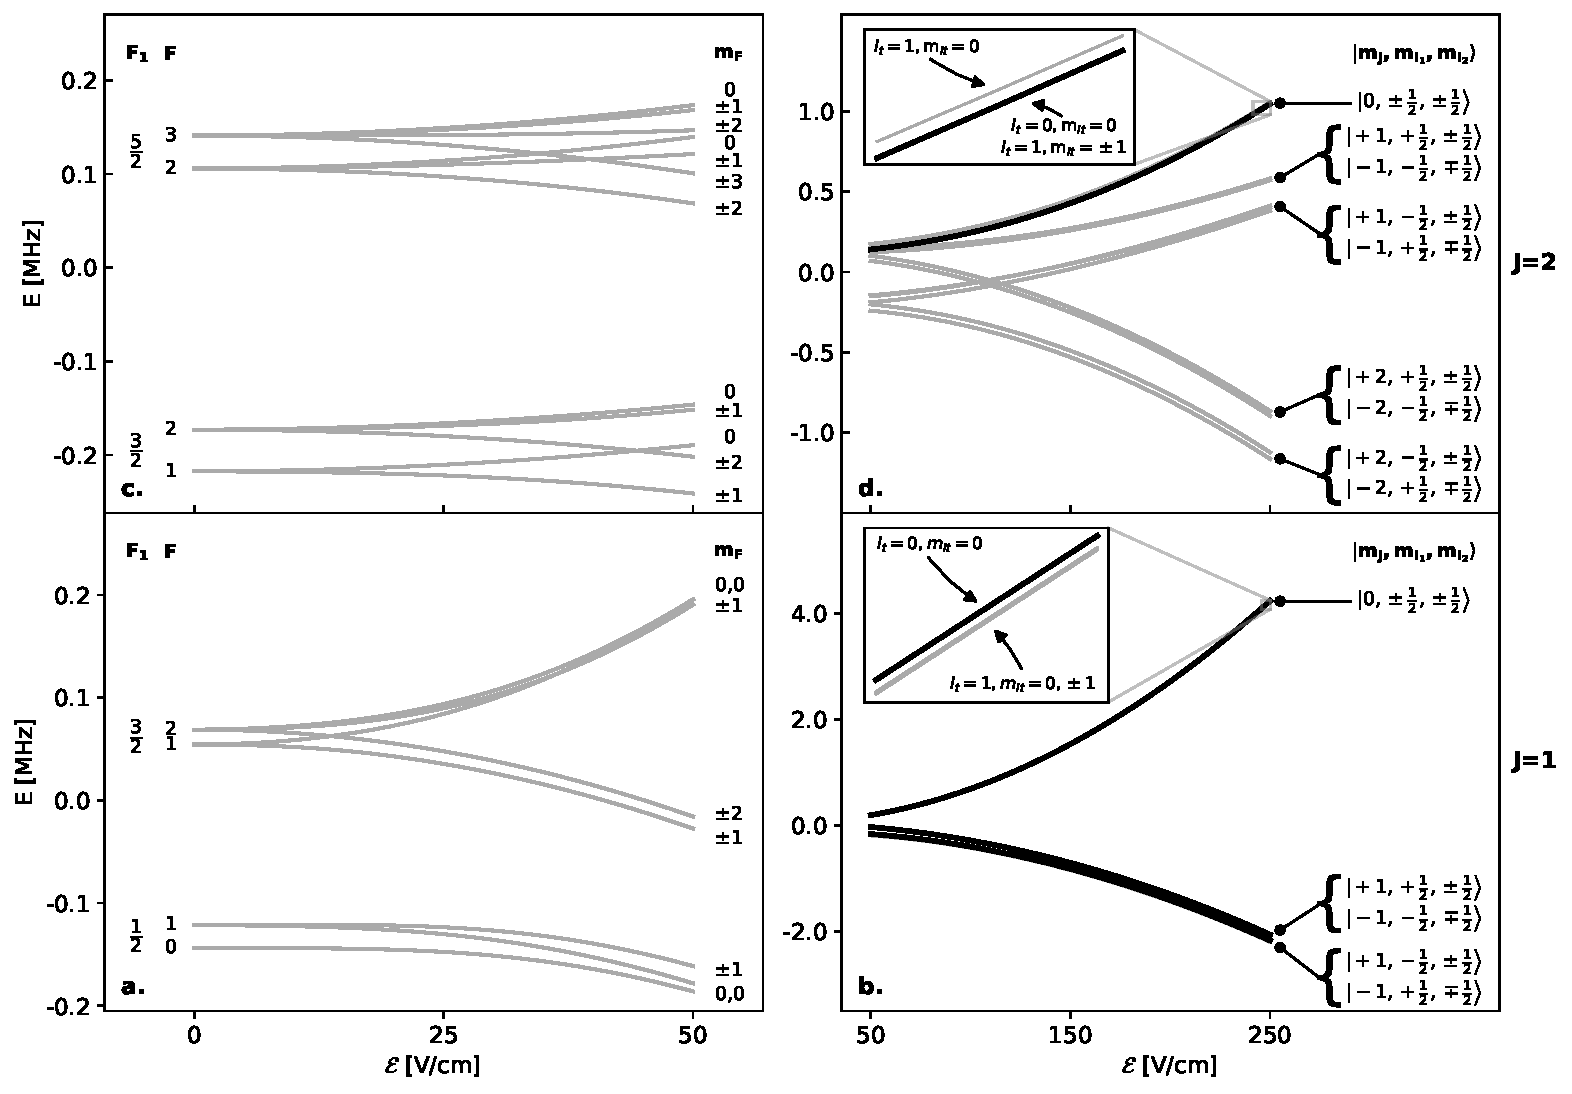
\includegraphics[width=\textwidth]{figs/matplotlib/low_to_mid_field.pdf}
	\caption{Overview of the energy eigenstates for changing $\Esca$-field magnitudes. The low-field regime, where $\Delta E_{\rm S} \ll E_{\rm hf}$, where energy eigenstates retain $J$, $F$, and $F_1$ as approximate quantum numbers is shown in \part{a} for $J=1$ and \part{c} for $J=2$. The mid-field regime, where $E_{\rm hf} \ll \Delta E_{\rm S} \ll E_{\rm rot}$, where both $J$ and $m_J$ are approximate quantum numbers is shown in \part{b} for $J=1$ and \part{d} for $J=2$. States used in \CENTREX\ are shown in bold.}
	\label{fig:low_to_mid_field}
\end{figure*}

\begin{figure}
	\centering
	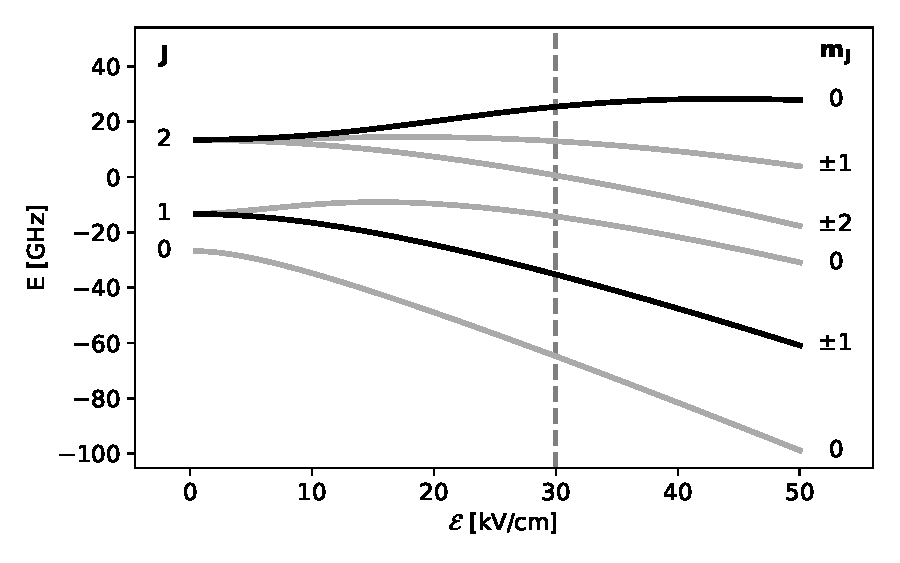
\includegraphics[width=\textwidth/2]{figs/matplotlib/low_to_high_field.pdf}
	\caption{Evolution of the energy eigenstates of the TlF Hamiltonian (Eq. \ref{eq:hyperfine_hamiltonian}) for $\Esca$ ranging from $0\,$V/cm to $50\,$kV/cm, for $J=0,1,2$. States used in \CENTREX\ are shown in bold. Hyperfine structure is unresolved in this plot.}
	\label{fig:low_to_high_field}
\end{figure}

Throughout most of the \CENTREX\ apparatus, TlF molecules experience a non-zero $\Esca$-field and (nominally) zero $\Bsca$-field.
The character of the energy eigenstates changes significantly depending on the $\Esca$-field magnitude, which varies dramatically between stages of the experiment. Hence, it is useful to describe the energy eigenstates of the TlF electronic ground state in different regimes of $\Esca$-field strength (with $\Bsca = 0$), as defined by the ratio of Stark shifts, $\Delta E_{\rm S} = \langle \mathcal{H}_{\rm S}\rangle \sim \mu_e^2 \Esca^2/B$, to the strength of hyperfine interactions, $E_{\rm hf} = \langle \mathcal{H}_{\rm sr} + \mathcal{H}_{\rm ss}\rangle \sim c_j$, or rotational energies, $E_{\rm rot} = \langle \mathcal{H}_{\rm rot}\rangle \sim B$. In all regimes, the total angular momentum projection $m_F$ along 
a space-fixed quantization axis $\hat{z}$ (always defined such that $\Evec$ is very nearly parallel to $\hat{z}$), is an exact quantum number.

In the low-field regime, where $\Delta E_{\rm S} \ll E_{\rm hf}$, energy eigenstates retain $J$, $F$, and $F_1$ as approximate quantum numbers. 
In the mid-field regime, where $E_{\rm hf} \ll \Delta E_{\rm S} \ll E_{\rm rot}$, both $J$ and $m_J$ are approximate quantum numbers. 
Here, the tensor part of the Stark shifts gives rise to energy splittings between levels with different values of $|m_J|$ that are comparable in size to the scalar shifts, i.e., of order $\Delta E_{\rm S}$.  Thus, when $m_J\neq 0$, $\vec{J}$ is strongly coupled to $\Evec$ (and hence to the molecular axis $\vec{\hat{n}}$) by this Stark interaction. In this case, each nuclear spin is coupled to $\vec{J}$ (and thus also to $\Evec$) by the spin-rotation interactions of $\mathcal{H}_{\rm sr}$. Hence, here $m_{I_1}$ and $m_{I_2}$ are approximate quantum numbers. By contrast, in states where $m_J=0$ (including when $J=0$) in this regime, $\left\langle \mathcal{H}_{\rm sr}\right\rangle$ vanishes to first order, and the nuclear spins do not couple to $\vec{J}$ and $\Evec$. However, the nuclear spins remain coupled to each other via the spin-spin interaction $\mathcal{H}_{\rm ss}$.  So, here the total nuclear spin $\vec \It = \vec I_1 + \vec I_2$ and its projection $m_{\It}$ are approximate quantum numbers in addition to $J$ and $m_J=0$. 
Finally, in the high-field regime where $E_{\rm hf} \ll E_{\rm rot} \lesssim \Delta E_{\rm S}$, $J$ states are strongly mixed, and separations between $m_J$ states are on the order of $E_{\rm rot}$. Here, eigenstates are defined by the same approximate quantum numbers as in the mid-field regime, aside from $J$. We refer to these strongly mixed states with the label $\widetilde{J}$, which corresponds to the value of $J$ that any given state connects to adiabatically, if the $\Esca$-field is reduced.
Table \ref{tab:E_field_regimes} summarizes the different regimes and associated eigenstates.  
\begin{table*}[t]
    \centering
    \def\colseplarge{4ex} % should only be used in this table
	\begin{tabular}{@{}r@{\hspace{\colseplarge}}r@{$\,\Delta E_{\rm S}\,$}l@{\hspace{\colseplarge}}r@{$\,\Esca\,$}l@{\hspace{\colseplarge}}>{\raggedright\arraybackslash}m{4cm}@{}}
    	\toprule
    	Regime & \multicolumn{2}{c}{Definition} & \multicolumn{2}{c}{Field strength} & Approx. eigenstates \\
		\midrule
		 Low
		 & & $\ll E_{\rm hf}$
		 & & $\lesssim 50 \Vcm$
		 & $\ket{J,F_1,F,m_F}$ \\\addlinespace[2ex]
		 %
	     Mid
	     & $E_{\rm hf} \ll$ & $\ll E_{\rm rot}$
	     & $50 \Vcm \ll$ & $\lesssim 5 \kVcm$
	     & $\ket{J,m_J \neq 0}\ket{m_{I_1},m_{I_2}}$ 
	       $\ket{J,m_J=0}\ket{\It,m_{\It}}$ \\\addlinespace[2ex]
	     %
	     High
	     & $E_{\rm hf} \ll E_{\rm rot} \lesssim$ &
	     & $5\kVcm \ll$ &
	     & $\ket{\widetilde{J},m_J\neq 0} \ket{m_{I_1},m_{I_2}}$
	       $\ket{\widetilde{J},m_J=0}\ket{\It,m_{\It}}$ \\
		\bottomrule
	\end{tabular}
	\caption{Regimes of electric field strength and associated eigenstates in TlF.}
	\label{tab:E_field_regimes}
\end{table*}


Figure \ref{fig:low_to_mid_field} shows how the relevant energies and eigenstates evolve from the low-field to the mid-field regime for $J=1$ and $J=2$ states.  Bold curves are states directly relevant to \CENTREX. Figure \ref{fig:low_to_high_field} shows a zoom out of states up to $J=2$ from low to high fields.

The $^{205}$Tl NSM measurement is carried out in $\tilde{J} = 1,\, m_J = \pm1$ states of TlF at large electric field $\mathcal{E} = 30$ kV/cm. This choice of states takes advantage of the structure of TlF in electric fields, in two ways. First, the observable energy shift associated with $S$, $\Delta E$, scales linearly with the degree of polarization $\mathcal{P}$ of the TlF molecule (Eq. \ref{eq:frequency_shift_due_to_NSM}). An electric field more easily polarizes states with low $J$, since $\mathcal{P}$ arises from mixing between states with different parity and thus different $J$; these states are closest together when $J$ is small. Additionally, as discussed in Sec. \ref{Sec:InternalComagnetometry}, certain dangerous systematic errors in the NSM measurement are dramatically suppressed in the presence of a strong spin-rotation interaction (later referred to as an effective intra-molecular magnetic field). This requires $m_J \neq 0$. The $\tilde{J} = 1,\, m_J = \pm1$ states hence provide the best combination of sensitivity and systematic error suppression in TlF.\footnote{$|\mathcal{P}|$ is larger in the $J=0,m_J = 0$ states, given the same $\Esca$-field value. Hence, the NSM gives larger energy shifts there. However, in these states where $m_J = 0$, the effective intra-molecular magnetic field vanishes.}
\section{Background}
\label{sec:background}

% \subsection{Meta-learning for speaker embeddings}

% \begin{itemize}
%     \item Includes protonets implementation “In defence of metric learning for speaker recognition” 
%     \item Talks about metric-learning (center loss?) “Comparison of metric-learning loss functions for E2E speaker verification” 
%     \item Protonets for short utterance speaker recognition 
%     \item \textbf{(Pending results)} Using deep clustering loss, based on spectral clustering: ||VVT - LLT||F 
% \end{itemize}

\subsection{Meta-Learning for Task Generalization}

Early works on meta-learning focused on adaptive learning strategies such as combining gradient descent with evolutionary algorithms \cite{yao_evolve1999,ABRAHAM20041}, learning gradient updates using a meta-network \cite{naik_metaNN1992} and using biologically inspired constraints for gradient descent \cite{bengio_synaptic1991, bengio1992optimization}.
Recent meta-learning approaches have addressed the issue of rapid generalization in deep learning, by learning to learn for a new task \cite{Andrychowicz_2016, finn_maml2017, ravi2017}.
This concept is inspired by the human ability to learn using a handful of examples. For instance children learn to recognize a new animal when presented with a few images as opposed to conventional DNNs which require thousands of samples for a new class.
The ability to quickly generalize to unseen classes is achieved by generating diversity in training tasks, for instance by using different sets of classes at each training step (see Fig. 1 in \cite{ravi2017}). Further, the classification setup (in terms of number of classes and samples per class) is controlled to match with that of the test task \cite{snell2017prototypical}.
Meta-learning has been successfully applied to achieve task generalization in computer vision \cite{ravi2017,snell2017prototypical,finn_maml2017} and more recently in natural language processing \cite{yu2018diverse,GaoH0S19, dou-etal-2019-investigating}.
Drawing parallels with the above applications, we train speaker embeddings with a large number of speaker classification tasks to improve over the conventional model which uses a single classification task. Since speaker sets differ between training steps, we replace the conventional softmax nonlinearity and cross-entropy loss combination with metric learning objectives used in previous meta-learning works \cite{snell2017prototypical,sung2018learning,vinyals2016matching,geng2019induction}.


\subsection{Meta-Learning Speaker Embeddings}

Few recent approaches have used a variant of meta-learning to train speaker embeddings, specifically the metric-learning objective from prototypical networks (protonets).
In \cite{chung2020defence}, the authors extend angular softmax objective to protonets and compare with various metric learning approaches for speaker verification. Across different architectures, angular prototypical loss outperforms other methods including conventional softmax objective. 
The authors in \cite{kye2020metalearning} applied protonets for short utterance speaker recognition and introduced global prototypes that mitigate the need for class sampling. 
In related applications, \cite{ko_protonets2020} and \cite{an2019shot} used protonets for small footprint speaker verification and few-shot speaker classification, respectively.
In \cite{wang_centroid2019}, the protonet loss was compared with triplet loss and evaluated on (open and close set) speaker ID and speaker verification tasks. 
However, previous approaches seldom compare embeddings trained using protonets with existing benchmarks based on x-vectors, except for \cite{ko_protonets2020} where a modified architecture was used owing to the nature of the task. Further, the class sampling strategy is not always used with protonets (e.g., \cite{chung2020defence,kye2020metalearning})
% triple-check above claim!)
which might inhibit task diversity during training. 
An exception from the above metric-learning approaches is \cite{kang2020domaininvariant}, where the authors train deep speaker embeddings using the model-agnostic meta-learning strategy to mitigate  domain mismatch for speaker verification.
To the best of our knowledge, meta-learning is yet to be applied for general-purpose speaker diarization, except for the specific case of dyadic speaker clustering in child-adult interactions in our recent work \cite{koluguri2020}. 

%> Protonets previously in speaker embedding applications
%> Connect relation networks to previous works, ones which learn the relation
% Refer to the Google Doc for a summary
\section{Methodology}
\begin{figure*}[t]
    \centering
    \scalebox{0.28}{
    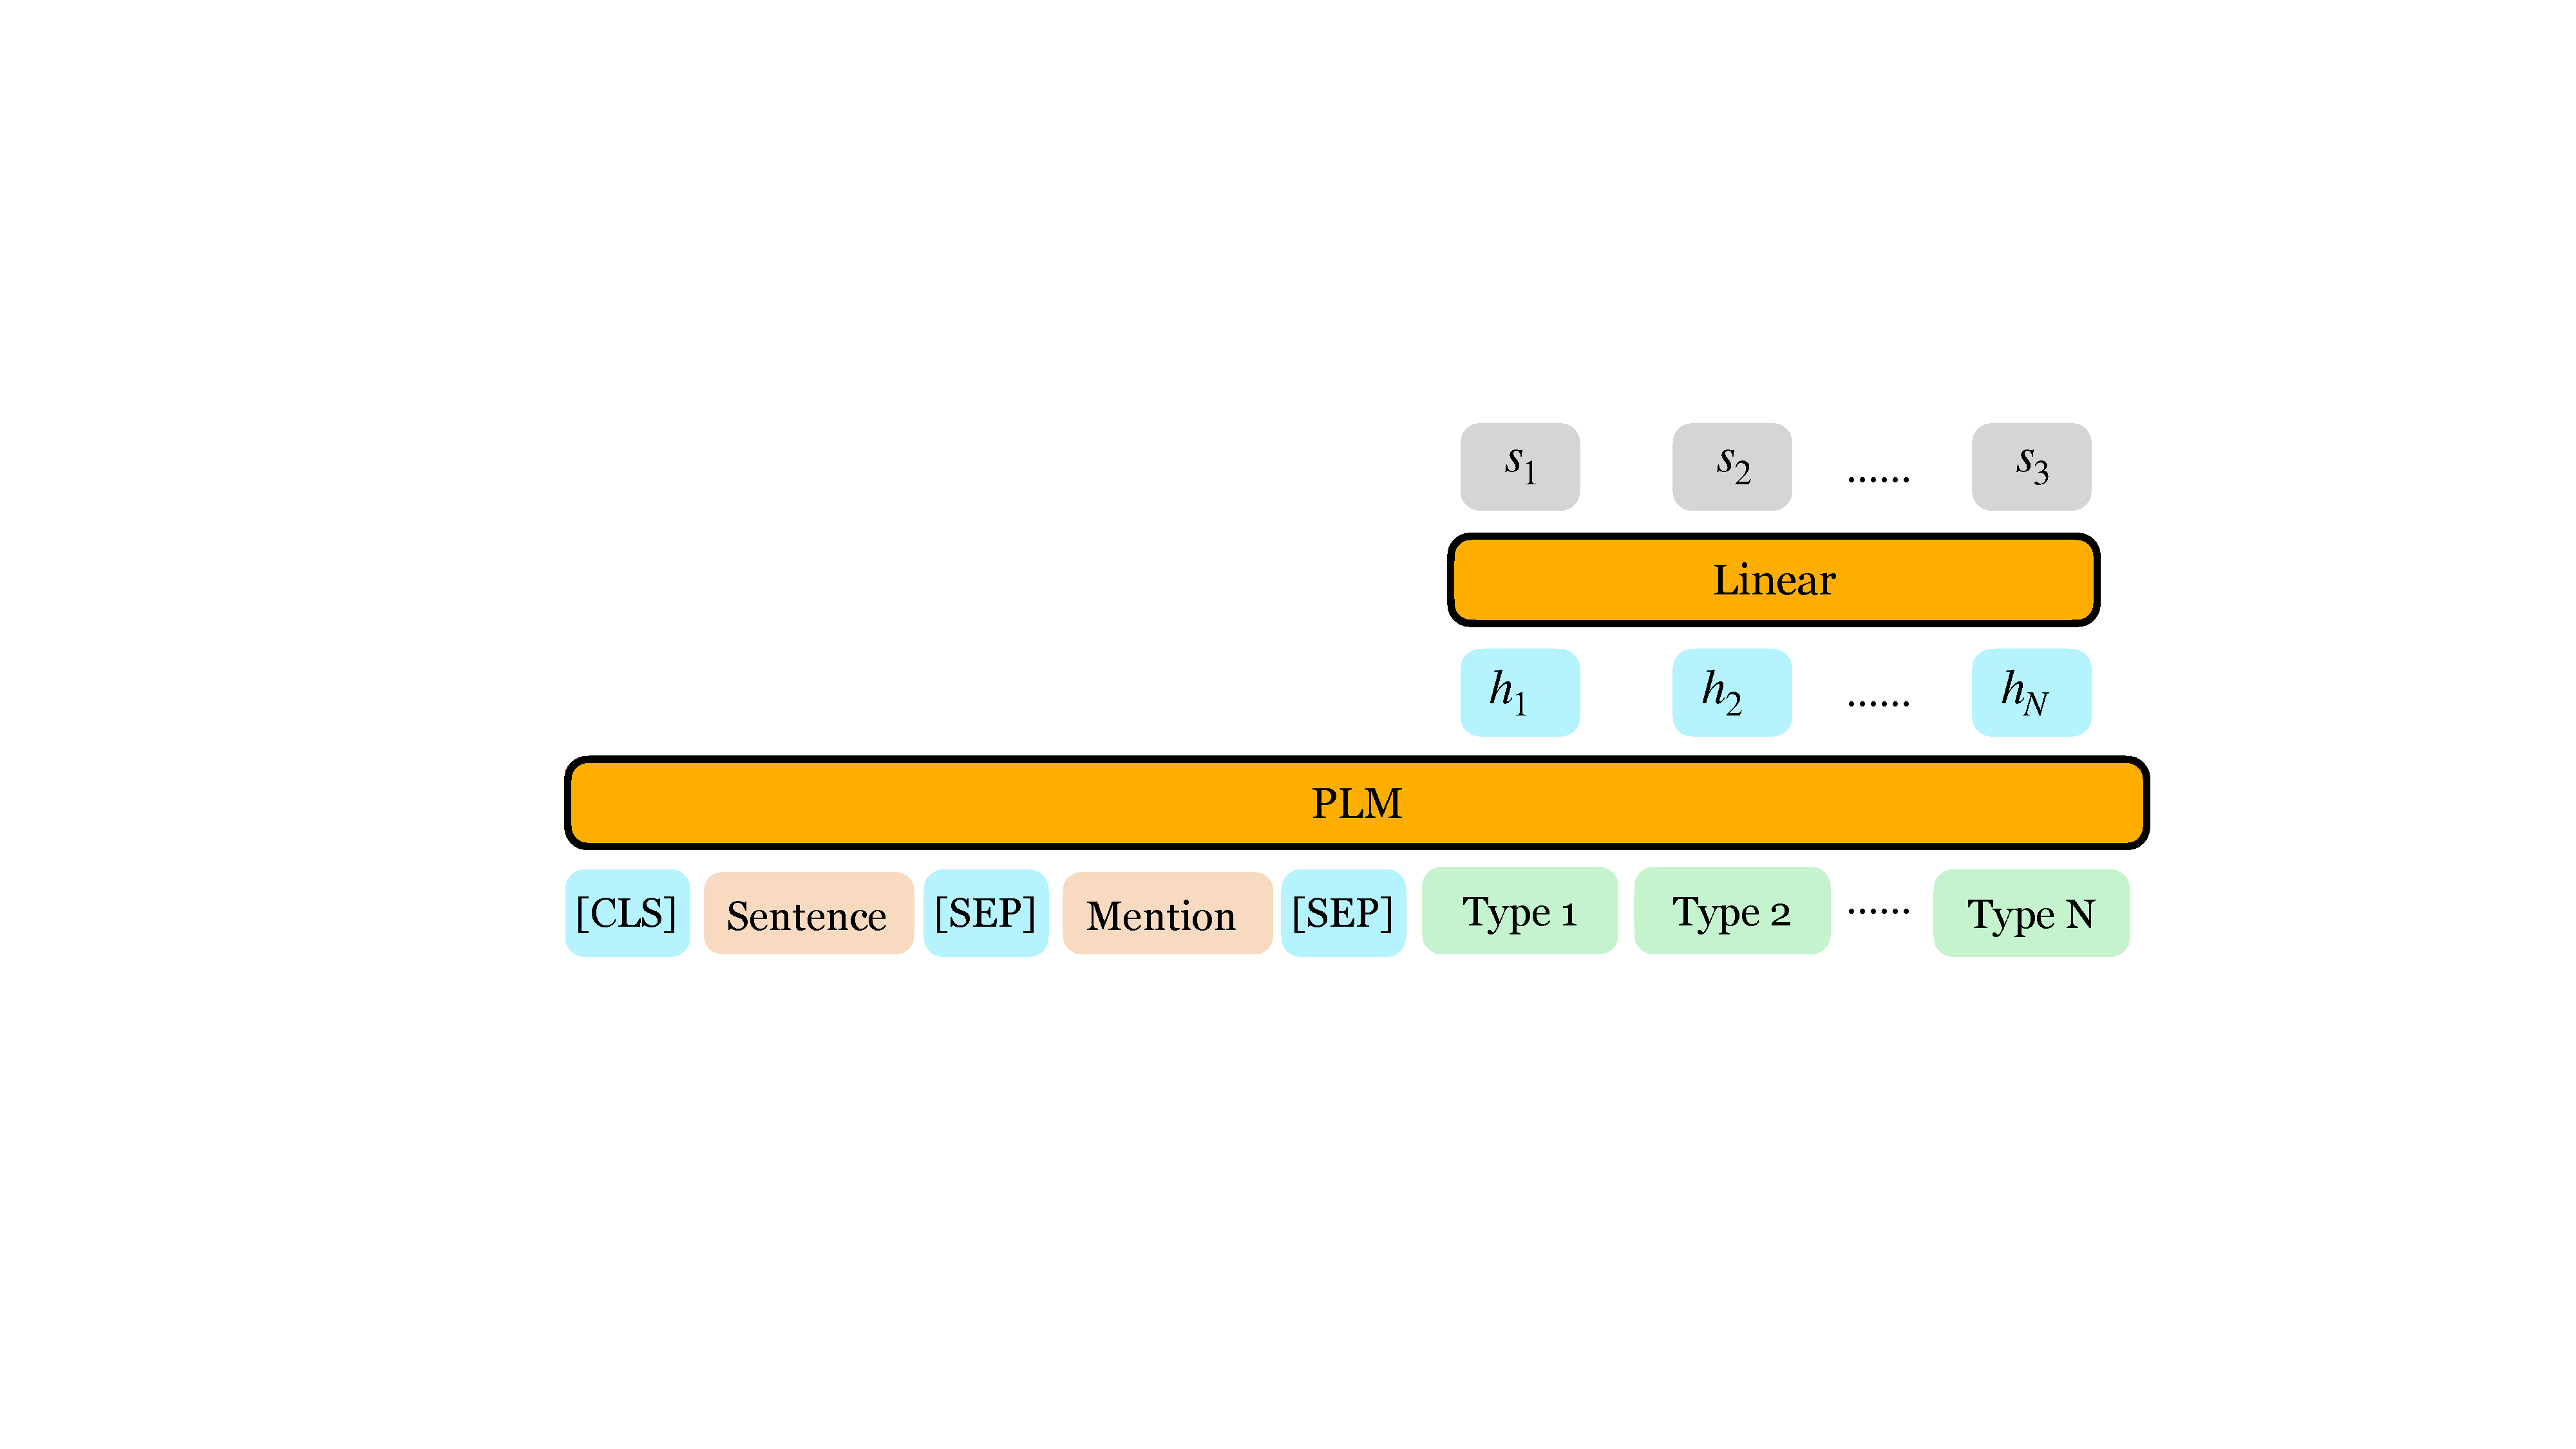
\includegraphics{src/img/ccf_model.pdf}}
    \caption{Multi-candidate cross-encoder (MCCE).}
    \label{fig:ccf}
\end{figure*}
Inspired by techniques in information retrieval \cite{ir} and entity linking \cite{wu2019zero}, we decompose the training and inference of UFET into three stages as illustrated in Figure \ref{fig:paradigm}: (1) Recall stage to reduce the type candidate size (e.g., from $N=10k$ to $K=100$) while guaranteeing the recall rate by an efficient MLC model. (2) Expand stage to incorporate lexical information using exact matching and weak supervision \cite{mlmet} from large pretrained language models such as BERT-Large \cite{bert} to improve recall rate. (3) Filter stage to filter the expanded type candidates to obtain final prediction. For the filter stage, we propose an efficient model: Multi-Candidate Cross-Encoder (MCCE) to concurrently encode and filter type candidates of a given mention with only a single forward pass. 
\subsection{Recall Stage}
To prune the type candidates set, we train a very efficient MLC model introduced in Sec. \ref{sec:mlc} and select the model based on the recall rate (e.g. recall@64) on the development set. Then we use it to infer the top $K_1$ (typically less than 256) candidates $\mathcal{C}_i^R$ for each data point $(m_i, c_i)$ for train, development, and test set. We compare MLC with a widely-used baseline model BM25 \cite{bm25} and show its advantages in Sec. \ref{sec:recall}. 
% There are other options (e.g., Bi-Encoder \cite{wu2019zero}) for the recall model. However, we choose MLC because it is easy to optimize and has the fastest inference speed\footnote{MLC model can be categorized as a simple Bi-Encoder that uses embedding to encode types.}.
\subsection{Expand Stage}
Due to the lack of training data per type, we found that the MLC we used in the recall stage easily overfits the train set, and is hard to predict the types that only appear in the development and test set. In {\bf \textsc{UFET}} dataset, 30\% of the types in the development set are unseen. To this end, we utilize lexical information using exact match and weak supervision from the masked language model (MLM) to expand the recalled candidates. Both exact match and MLM are able to recall unseen type candidates without any training. 
\paragraph{Exact Match} MLC and Bi-Encoder recall candidates by dense representations. They are known weak at identifying and utilizing the lexical matching information between the input and types \cite{matching_info1, matching_info2}. However, 
 types are free-formed in UFET (e.g., \textit{president, businessman}), and are very likely to appear in the context or mention (e.g., the mention is \textit{`the \textbf{president} Joe Biden'}). To this end, we first find all nouns in the context and mention by NLTK\footnote{nltk.tag package \url{https://www.nltk.org}} POS tagger and normalize their forms, then we recall types that exactly matched with these nouns.
\paragraph{Weak Supervision from MLM} Inspired by recently prompt-based methods for entity typing \cite{ding2021prompt, dfet}, we recall candidates by asking PLMs to fill masks in prompts. Suppose a type $y_j \in \mathcal{Y}$ can be tokenized into $l$ subwords $w_1, \cdots w_l$. To score $y_j$ given $m_i, c_i$, we first formulate the input as in Figure \ref{fig:prompt_recall}.
\begin{figure}[h]
    \centering
    \scalebox{0.2}{
    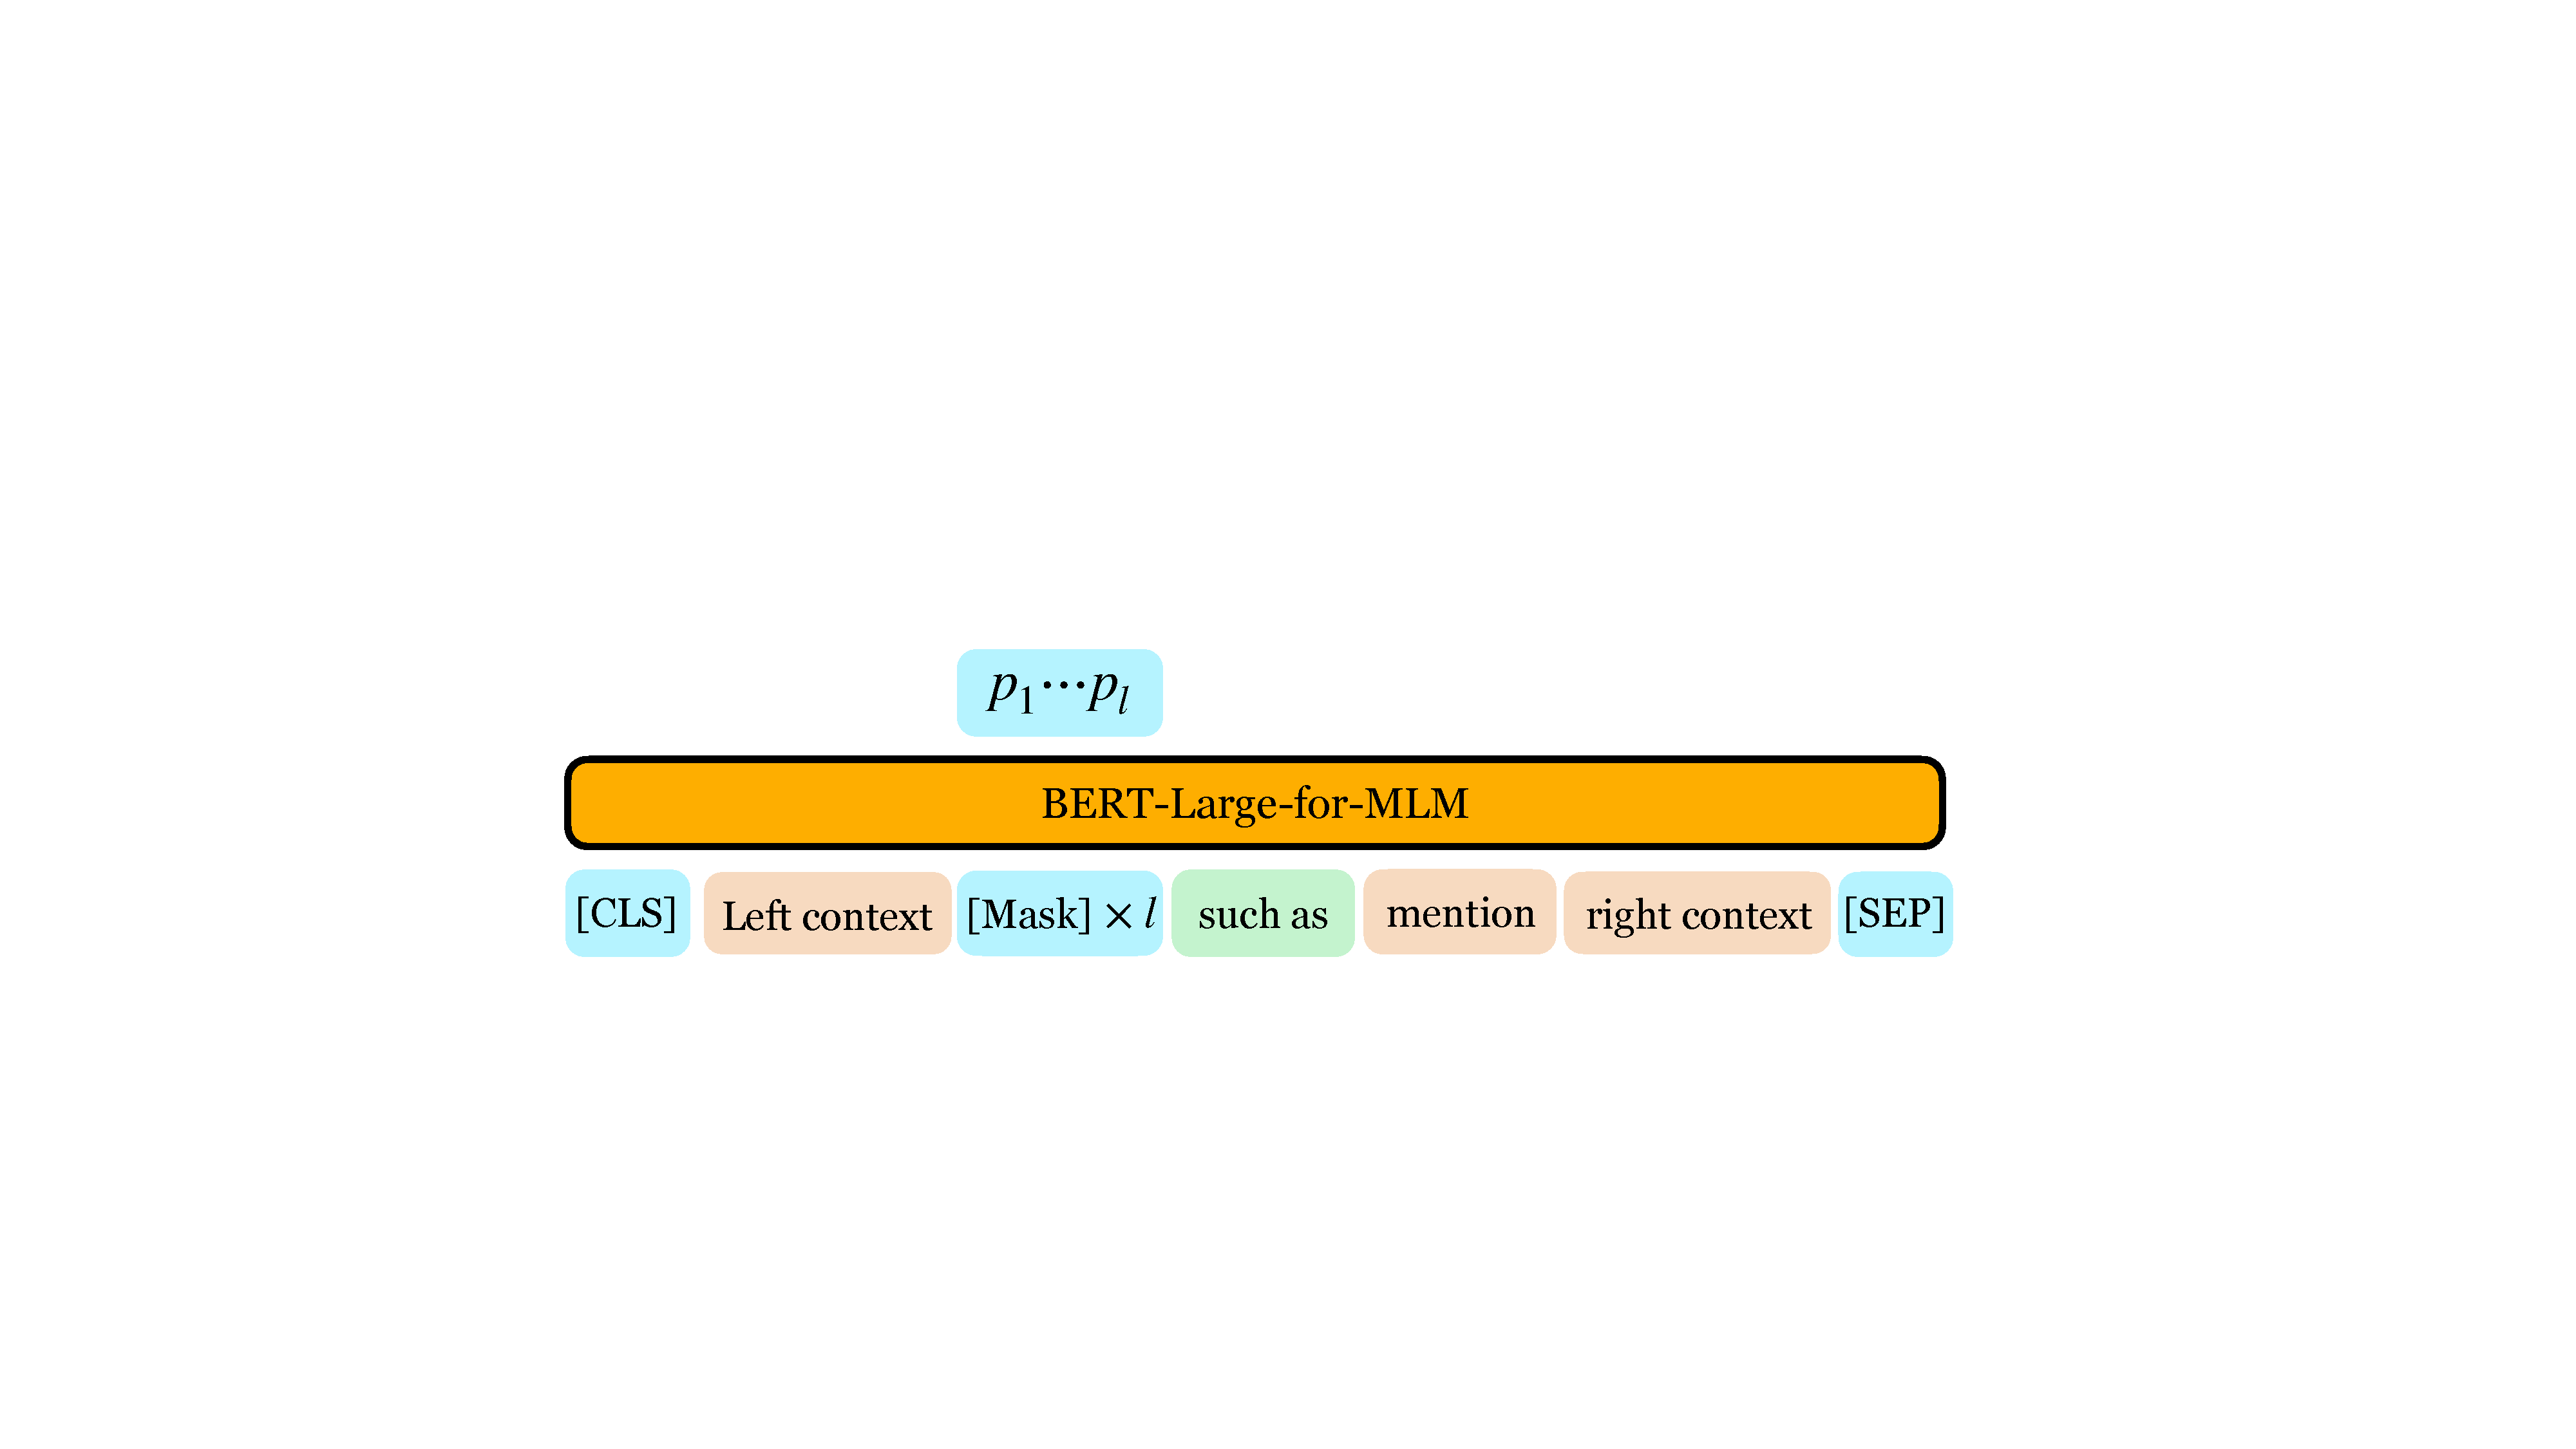
\includegraphics{src/img/prompt_recall.pdf}}
    \caption{Recall from MLM using prompts.}
    \label{fig:prompt_recall}
\end{figure}
where $c_i^l, c_i^r$ are left and right context of $m_i$, and \texttt{`such as'} is the template we use to induce types. The input is then fed into BERT-large-uncased\footnote{We use the PLM from \url{https://huggingface.co}} for masked language model to obtain the probabilities of subwords, the score of $y_j$ is calculated by $ s^{MLM}_{j} = (\sum_{n=1}^l \log p_n)/l$, where $p_l$ denotes the probability of subword $w_l$ predicted by the PLM. We rank all types by enumerating all possible $l$ and recall $K_2$ additional candidates that haven't been recalled by the recall stage and exact match. We found that the expand stage improves recalls and contributes to the performance in Sec. \ref{sec:exp_expand}.
\subsection{Filter Stage}
In the filter stage, we use the recall and expand method introduced above to efficiently generate type candidates $\mathcal{C}_i$ for data in the train, development, and test set. For training, $\mathcal{C}_i$ is used to produce positive and hard negative type candidates. For inference, $\mathcal{C}_i$ is the candidate pool for the trained filter models. Let $|\mathcal{C}_i|=K$ and $K$ is typically less than 256. 
\subsubsection{CE} A trivial idea is to train a CE model introduced in Sec. \ref{sec:vanilla_ce} to filter $\mathcal{C}_i$ instead of filtering the whole type set $\mathcal{Y}$. The positive type $y^{+}$ and negative $y^{\_}$ type are both sampled from $\mathcal{C}_{i}$ and are used for calculating marginal ranking loss. To infer types, we also recall and expand $K$ candidates and score these candidates by $K$ forward passes to predict types. As $K << |\mathcal{Y}|$, CE with our Recall-Expand-Filter paradigm is much faster than vanilla CE. However, it's still inefficient compared to MLC-like models that concurrently predict scores of all types in a single forward pass. For faster inference and training, we propose multi-candidate cross-encoders ({\bf \textsc{\name}}) and introduce them in the next section.

\section{Multi-Candidate Cross-Encoder (\name)}
\label{sec:ccf}
 In this section, we introduce {\bf \textsc{\name}} for filtering candidates in one forward pass and propose several variants. 
\subsection{Overall Introduction of \name}
As shown in Figure \ref{fig:ccf}, compared to CE that concatenates one candidate at a time, {\bf \textsc{\name}} models concatenate all candidates in $\mathcal{C}_i$ with the mention and context. The input is then fed into the PLM to obtain the hidden states of each candidate as their representation. Finally, we use an MLP to concurrently score all candidates.
\begin{equation}
\begin{aligned}
\bm{h}_{1:K}  &= \texttt{PLM}(\texttt{[CLS]} \ c_i \ \texttt{[SEP]}\  m_i \ \texttt{[SEP]} \ t_{1:K} \ )  \\
\bm{s}_{1:K}  &= \texttt{Linear}(\bm{h}_{1:K}) 
\end{aligned}
\end{equation}
where $t_{1:K}$ is the short for $t_1, \cdots, t_K$, and $t_j \in \mathcal{C}_i$. Similarly, $\bm{h}_{1:K}$ and $s_{1:K}$ are hidden representations and scores of corresponding candidates respectively. 

\paragraph{Training and Inference} For training, we found that all positive types are ranked very high in the training candidates, which is not the case for the development and test data. To prevent the filter model from overfitting the order of training candidates and only learning to predict the first several candidates, we keep permuting type candidates during training. Same as the MLC model mentioned in Sec. \ref{sec:mlc}, we use the Binary Cross-Entropy loss as the training objective and tune a threshold of probabilities on the development set for inference.

In the next subsection, we discuss different model configurations of {\bf \textsc{\name}} regarding the input formats of candidates and attention mechanisms.

\subsection{Different Input Formats of Candidates}
\paragraph{Average of type sub-tokens} We treat each type $t_j \in \mathcal{Y}$ as a new token $u_j$ and add it to the vocabulary of PLM. The static embedding (layer 0 embedding of PLM) of $u_j$ is properly initialized by the average static embedding of $t_j$'s sub-tokens. As type candidates are capsuled into single tokens, the candidate representation $t_j$ is simply the last hidden state of $u_j$. The reasons for representing each type as a single token is (1) The max sequence length allowed by most PLMs is limited to 512, compressing types into single tokens is position saving. (2) Types in {\bf \textsc{UFET}} are tokenized into $2.1$ sub-tokens in average (by RoBERTa's tokenizer). Compressing types will not lose too many type semantics.
\paragraph{Fixed-size sub-token block} To preserve more type semantics, we place each candidate into a fixed-sized block as shown in Figure \ref{fig:cand_block}. We found the fixed block size makes PLM easier to enable the parallel implementation of different attention mechanisms that we will introduce next. We use the first hidden state in the block as the candidate representation.
\begin{figure}[h]
    \centering
    \scalebox{0.3}{
    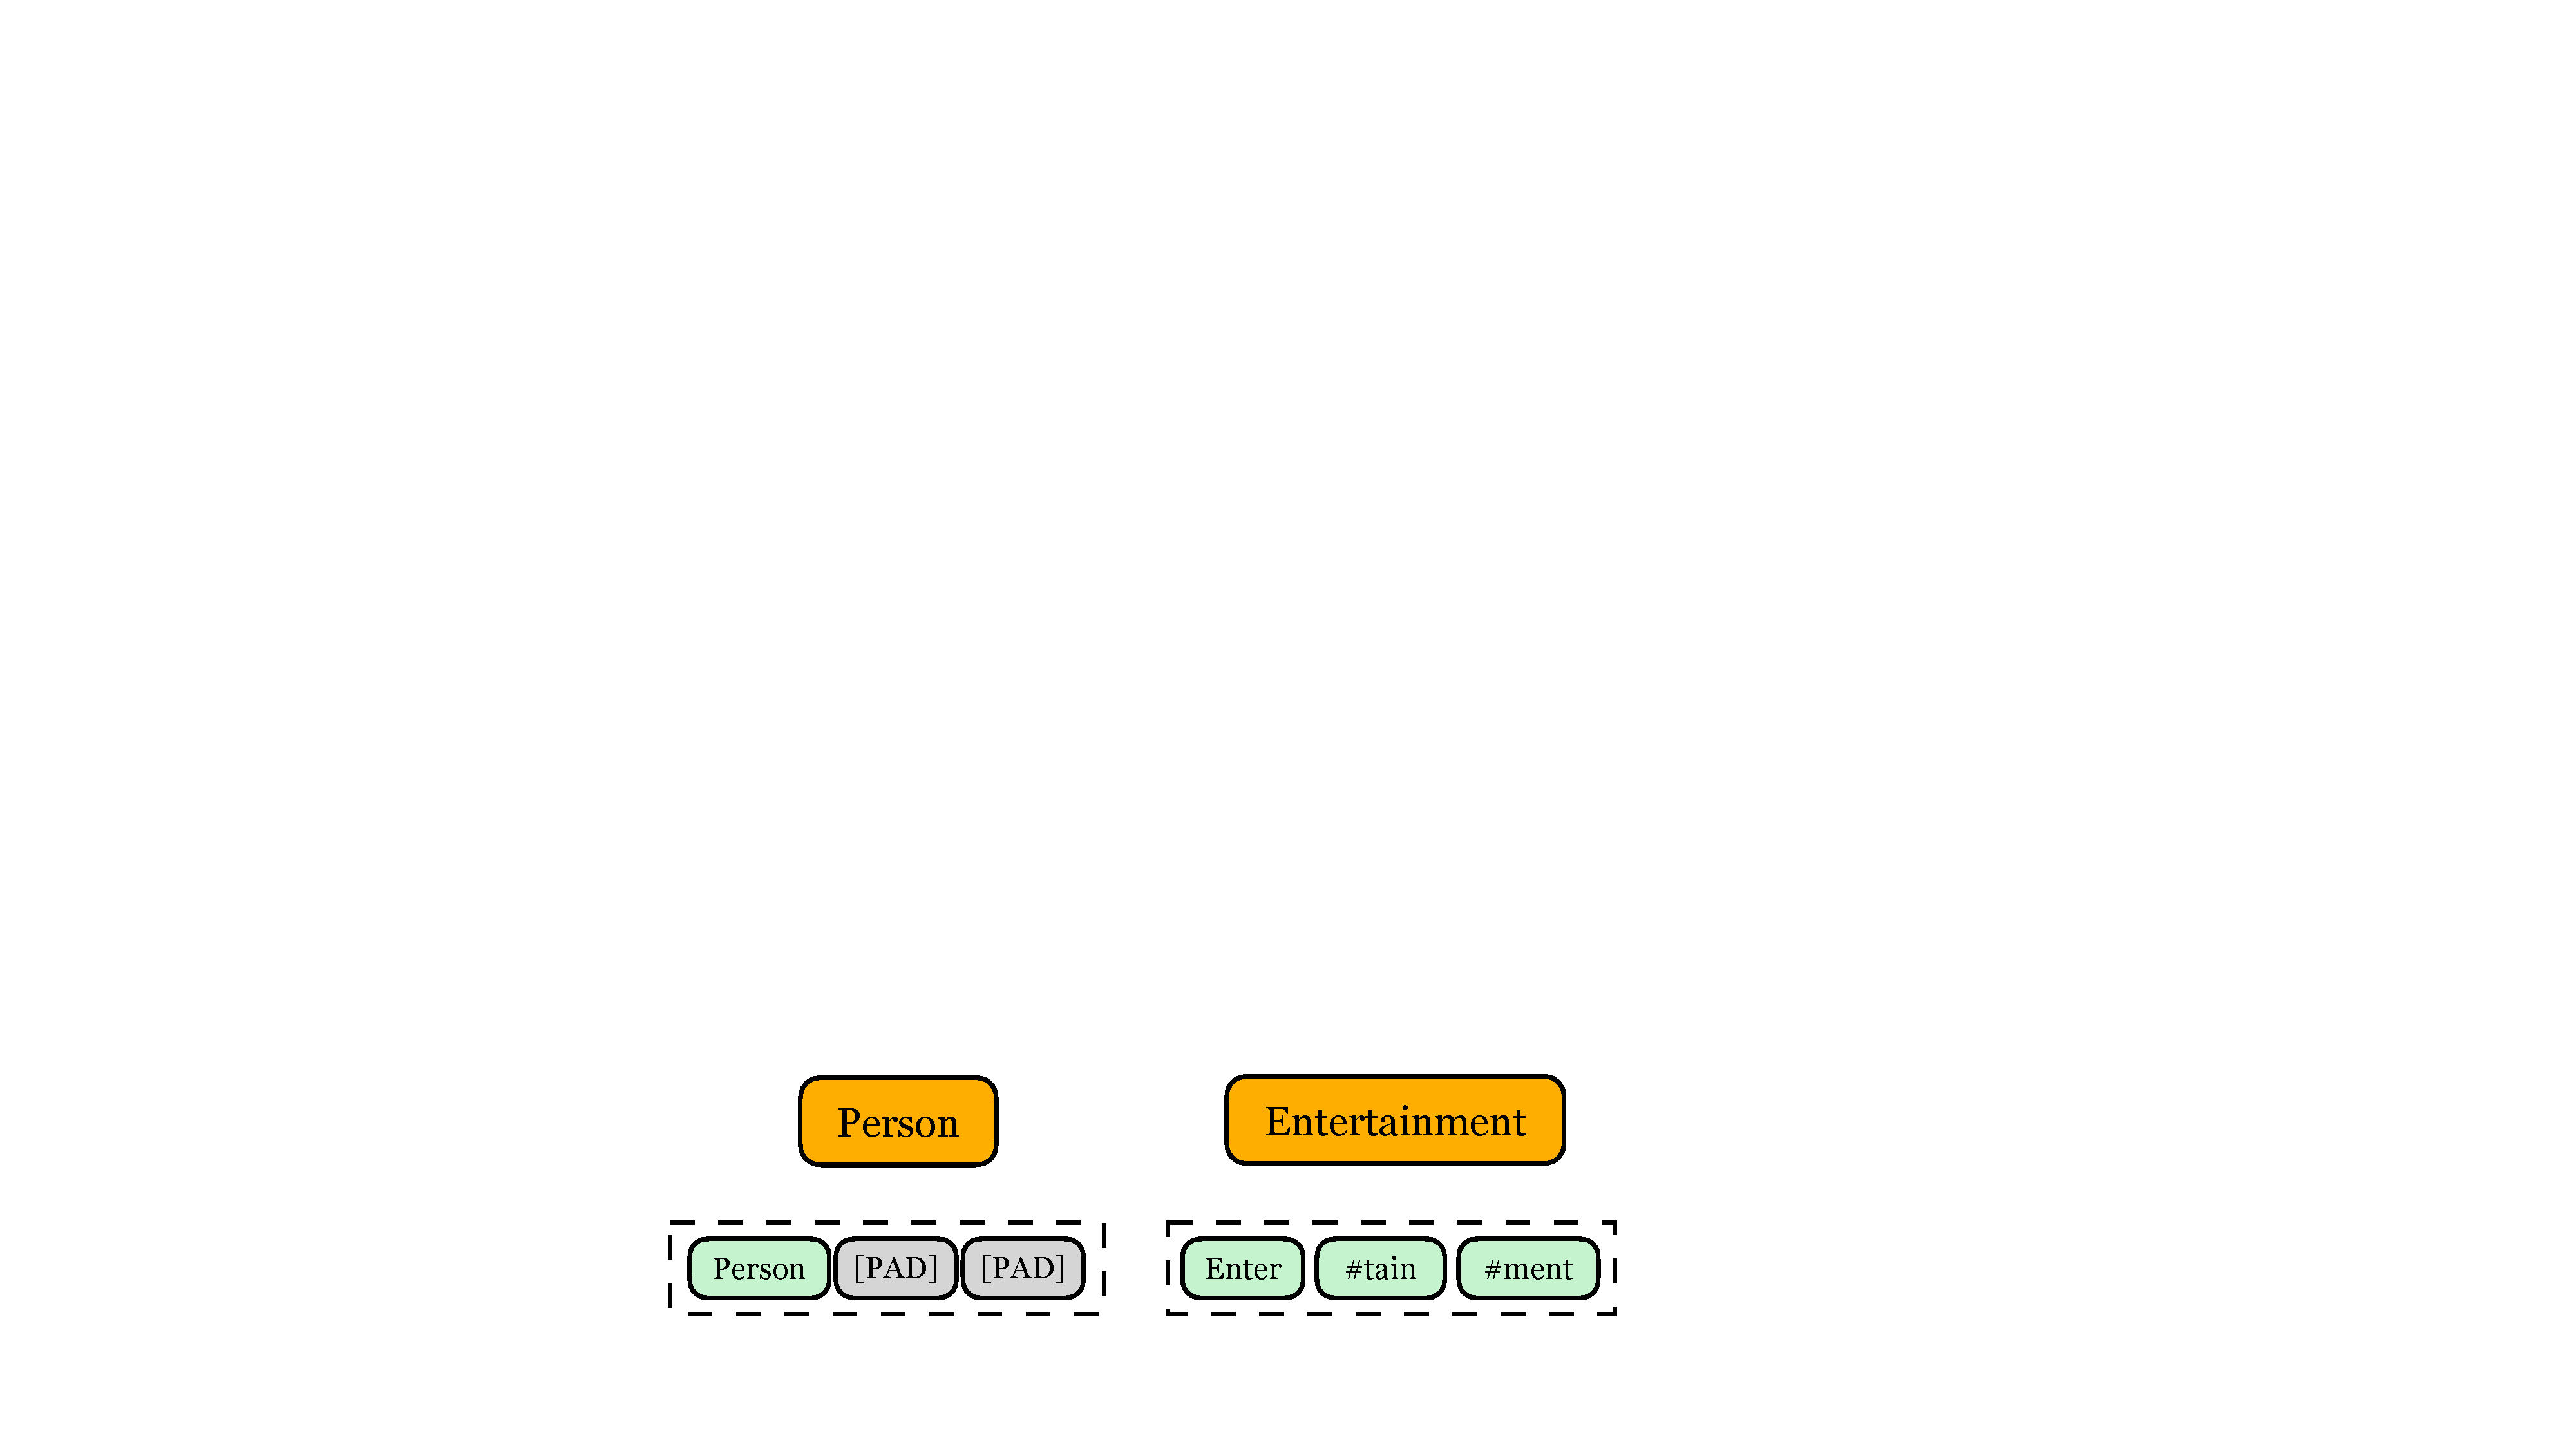
\includegraphics{src/img/cand_block.pdf}}
    \caption{Illustration of candidate block.}
    \label{fig:cand_block}
\end{figure}

\subsection{Attentions in \name}
\label{sec:attn}
There are four kinds of attention in {\bf \textsc{\name}} as shown in Figure \ref{fig:attn1}, sentence to sentence (S2S), sentence to candidates (S2C), candidate to sentence (C2S), and candidate to candidate (C2C). As we score candidates based on mention and its context, attention from candidates to the sentence (C2S) is necessary. However, the necessity of C2C, S2S, and S2C is questionable. As our analytical experiment in Sec. \ref{sec:analyze} shows, it is important for words in the sentence to attend to all candidates (S2C), and is useful to have self-attention in the sentence (S2S), but the attentions (C2C) between different candidates are unnecessary. Based on these findings, we propose a new variant of {\bf \textsc{\name}} that the C2C attention is discarded in computation as shown in the right part of Figure \ref{fig:attn1}. Let $L_S$ and $L_C$ be the number of sub-tokens used by the sentence and candidates respectively. We can formulate the attention query of the sentence as $\bm{Q}_S=[\bm{q}^s_{1};\cdots;\bm{q}^s_{L_S}] \in \mathbb{R}^{L_S \times D}$,  where $\bm{q}^s_i$ is the query vector of the $i$-th sub-token in the sentence, and $D$ is the embedding dimension. Similarly, the query of candidates is formulated as $\bm{Q}_C=[\bm{q}^c_{1};\cdots;\bm{q}^c_{L_C}] \in \mathbb{R}^{L_C \times D}$. When we treat candidates as average of sub-tokens, $\bm{q}^c_i$ is a $D$-dimensional vector, and when we use fixed-sized blocks to place candidates, $\bm{q}^c_i \in \mathbb{R}^{B \times D}$ is the concatenation of the query vectors in the $i$-th candidate block and $B$ is the number of sub-tokens in a block. The keys and values are defined similarly as $\bm{K}_C, \bm{V}_C, \bm{O}_C \in \mathbb{R}^{L_C \times D},  \bm{K}_S, \bm{V}_S, \bm{O}_S \in \mathbb{R}^{L_S \times D}$. The attention outputs are computed as:
\begin{align}
& \bm{O}_S  = \text{Softmax} \big( \frac{\bm{Q}_S [\bm{K}_S; \bm{K}_C]^T}{\sqrt{D}} \big) \cdot [\bm{V}_S; \bm{V}_C] \\
&[\bm{A}_{CS}; \bm{A}_{CC}]  = \text{Softmax} \big( \frac{[\bm{Q}_C \bm{K}_S^T; \bm{M}_C^T]}{\sqrt{D}} \big)  \\
&\bm{M}_C  =  [{\bm{q}_1^c}^T \bm{k}_1^c; \cdots; {\bm{q}_{L_C}^c}^T \bm{k}_{L_C}^c] \\
&\bm{A}_{CC} = [\bm{a}^c_{1}; \cdots; \bm{a}^c_{L_C}] \\
&\bm{O}_C = \bm{A}_{CS} \bm{V}_S + \sum_{j=1}^{L_C} \bm{a}_j \bm{v}^c_j
\end{align}
where $\bm{A}_{CC}$ is the intra-candidate or intra-block attention, and $\bm{a}_j^c$ is a scaler when we treat candidates as average of sub-tokens and is a $B \times B$ matrix when we represent candidates as blocks. The last step (Eq. 8) can be parallelly implemented by Einstein summation.
In most cases, candidate length $L_C$ is significantly larger than sentence length $L_S$. As a result, by ignoring the C2C attention, the inference speed is further improved because the time complexity of the attention is significantly reduced from $O(D(L_S+L_C)^2)$ to $O(D(L_S^2+2L_SL_C+B^2L_C))$. More importantly, the space complexity in attention also gets reduced from $O((L_S+L_C)^2)$ to $O(L_S^2+2L_SL_C))$, which allows us to filter more candidates concurrently. The improvement in space and time complexity by discarding C2C attention is more obvious when the number of candidates becomes larger.

\begin{figure}[h]
    \centering
    \scalebox{0.22}{
    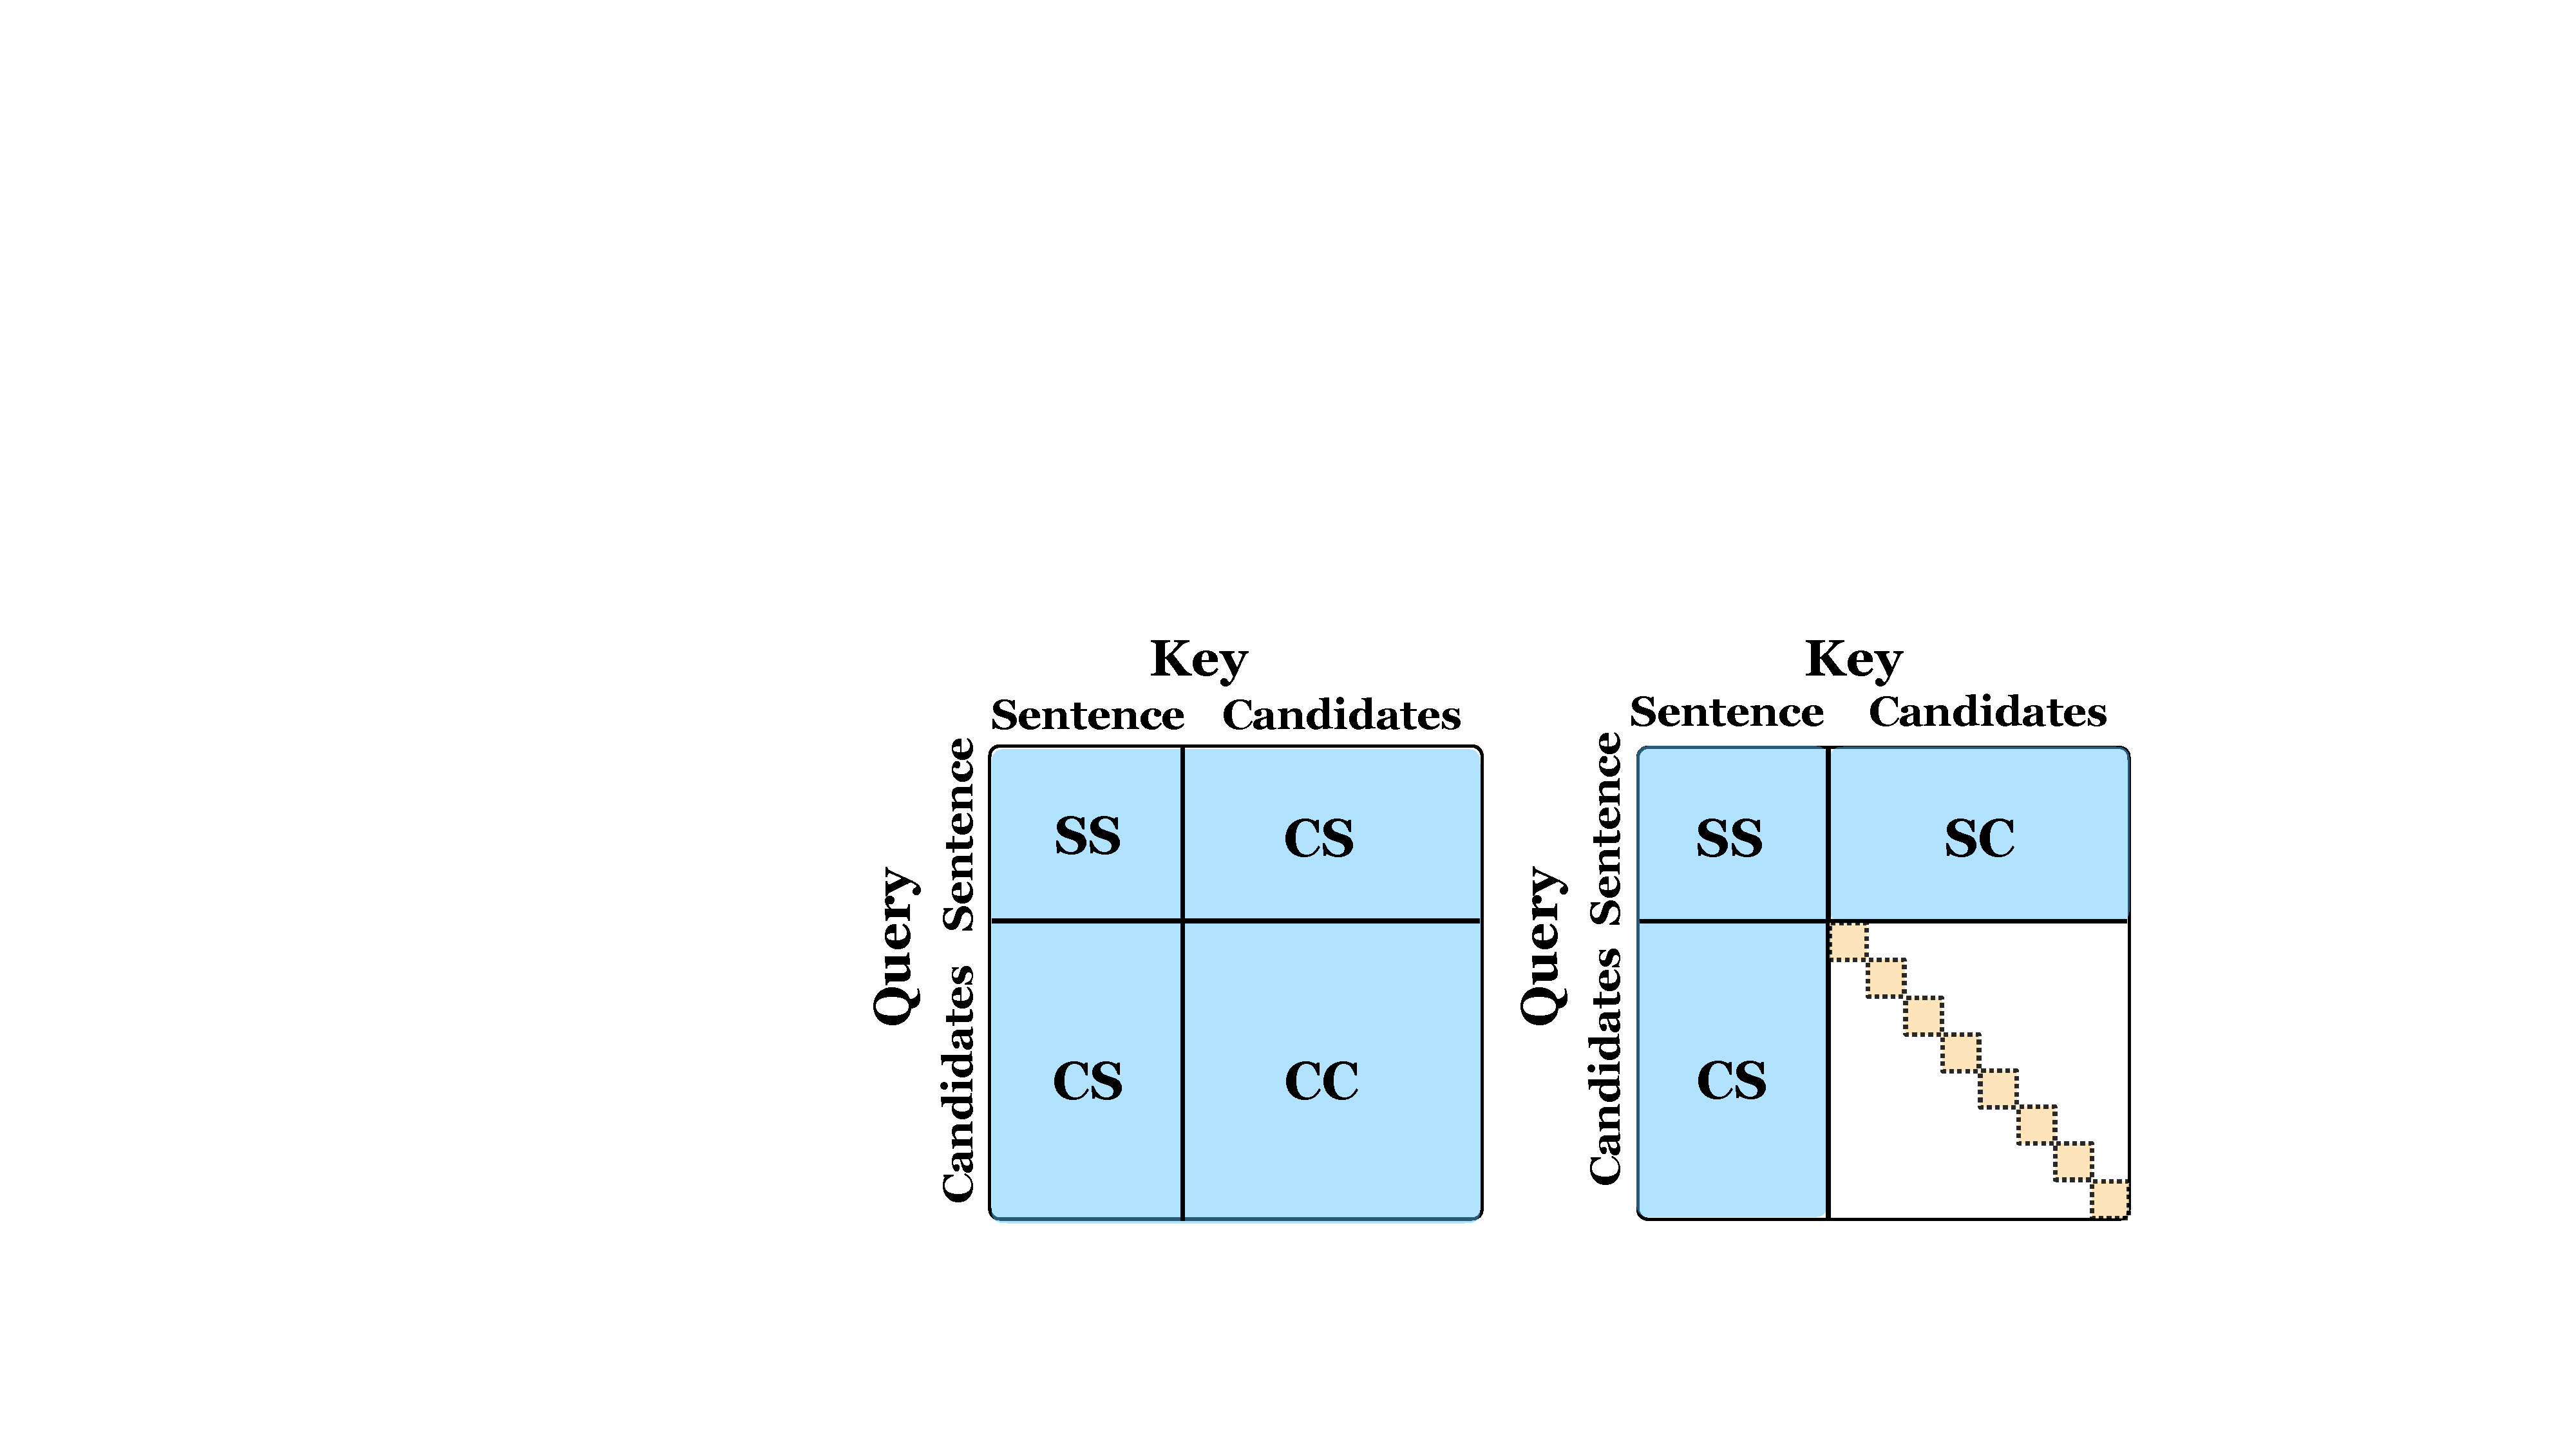
\includegraphics{src/img/attn_all.pdf}}
    \caption{Attentions in {\bf \textsc{\name}} (left), and {\bf \textsc{\name}}  without candidate-to-candidate (C2C) attention (right).}
    \label{fig:attn1}
\end{figure}
\section{Experiments}
We conduct experiments on two ultra-fine entity typing datasets, {\bf \textsc{UFET}} (English) and {\bf \textsc{CFET}} (Chinese). Their data statistics are shown in Table \ref{tab:stat}. We mainly focus on and report the macro-averaged recall at the recall and expand stage, and concern mainly on the macro-$F1$ of the final prediction at the filter stage. We also evaluate the {\bf \textsc{\name}} models on the fine-grained (130 types) and coarse-grained (9 types) settings of entity typing without the recall and expand stage.
\subsection{UFET and CFET}
\subsubsection{Recall Stage}
\label{sec:recall}
We compare the recall@$K$ on the test sets of {\bf \textsc{UFET}} and {\bf\textsc{CFET}} between the trained MLC model (introduced in \ref{sec:mlc}) and a traditional BM25 model \cite{bm25} in Figure \ref{fig:recall}. The MLC model uses the RoBERTa-large as backbone and is tuned based on the recall@$128$ on the development set. We use AdamW optimizer with a learning rate of $2\times10^{-5}$. Results show that MLC is a strong recall model, it consistently has better recall compared to BM25 on both {\bf\textsc{UFET}} and {\bf\textsc{CFET}} dataset, and the recall@$128$ reaches over $85\%$ on {\bf \textsc{UFET}}, and over $94\%$ on {\bf \textsc{CFET}}.

\begin{figure}[t]
     \centering
     \begin{subfigure}[h]{0.5\textwidth}
         \centering
         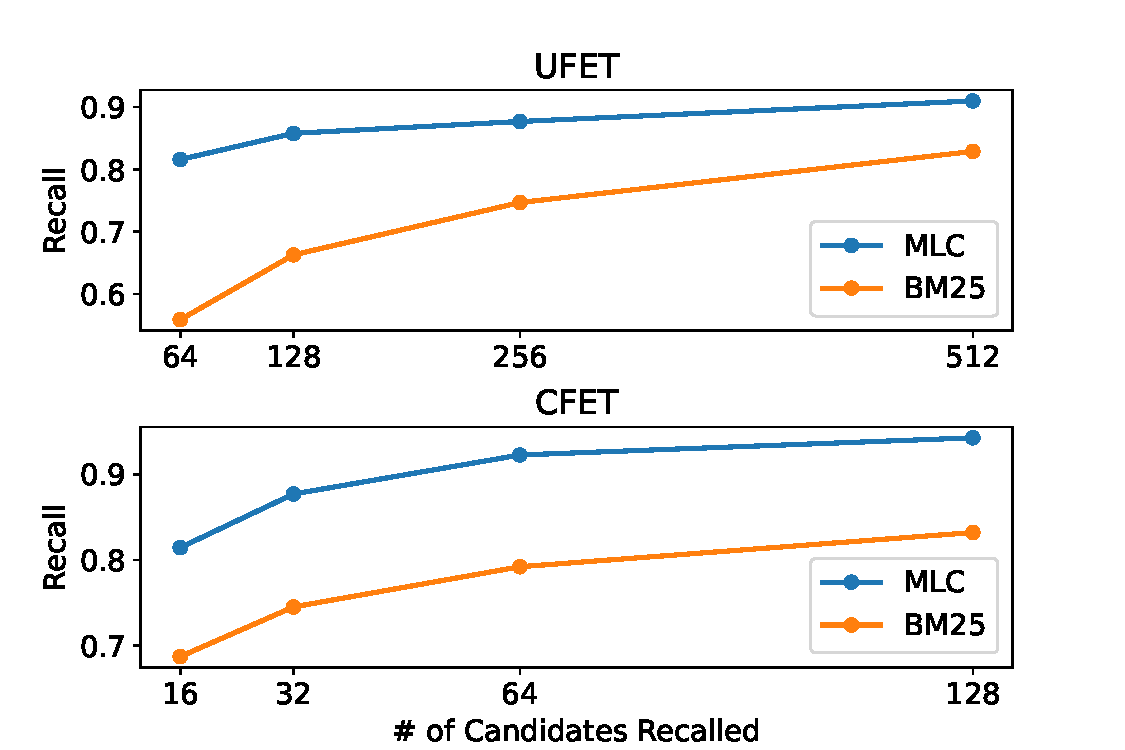
\includegraphics[width=\textwidth]{src/img/recall_compare_bm25.pdf}
         \label{fig:mb2}
     \end{subfigure}   
 \caption{Recall@$K$ of MLC and BM25.}
 \label{fig:recall}
\end{figure}

\subsection{Expand Stage}
\label{sec:expand}
In Table \ref{tab:expand}, we evaluate the F1 scores of all candidates expanded by exact match, and top-$10$ candidates expanded by the MLM using Bert-large. We also demonstrate the improvement of recall by using candidate expansion in Figure \ref{fig:expand_improvement}. On {\bf \textsc{UFET}} dataset, expanding around $32$ additional candidates based on $112$ MLC candidates results in $2\%$ higher recall compared to recalling all $128$ candidates by MLC. The recall of $128$ candidates after the expansion is comparable to the recall of $180$ candidates recalled from MLC. Similarly, expanding $10$ candidates is comparable to additionally recalling $80$ candidates using MLC.
In our experiments, we replace the last $48$ candidates recalled by MLC with the candidates recalled by MLM and Exact match for {\bf \textsc{UFET}} and $10$ for {\bf \textsc{CFET}}. We found the expand stage has a positive effect on the final performance of {\bf \textsc{\name}}s, and helps them reach SOTA performance (analyze in Sec. \ref{sec:analyze}).


\begin{table}[t]
\centering
\scalebox{0.75}{
\begin{tabular}{cccccc} 
\toprule
{\bf \textsc{Dataset}} & {\bf \textsc{Expand}} &   {\bf \textsc{P}}  & {\bf \textsc{R}}  &  {\bf \textsc{F1}} & \small{Avg \# Expanded}  \\ \midrule
\multirow{2}{*}{\bf \textsc{UFET}} & {\bf \textsc{Match}}      & 11.2   & 11.3     & 9.8    & 5.23     \\
      & {\bf \textsc{MLM}}  &  8.5     &   17.1   &  10.7  &    10    \\ \midrule
\multirow{2}{*}{\bf \textsc{CFET}} & {\bf \textsc{Match}}   &  11.4  &  14.5  & 11.2   & 4.57    \\
 & {\bf \textsc{MLM}}  & 21.3   &  19.5  & 17.7    & 10    \\ \midrule
\end{tabular}}
\caption{Evaluation of the recalled candidates.}
\label{tab:expand}
\end{table}
\begin{figure}[t]
     \centering
     \begin{subfigure}[h]{0.45\textwidth}
         \centering
         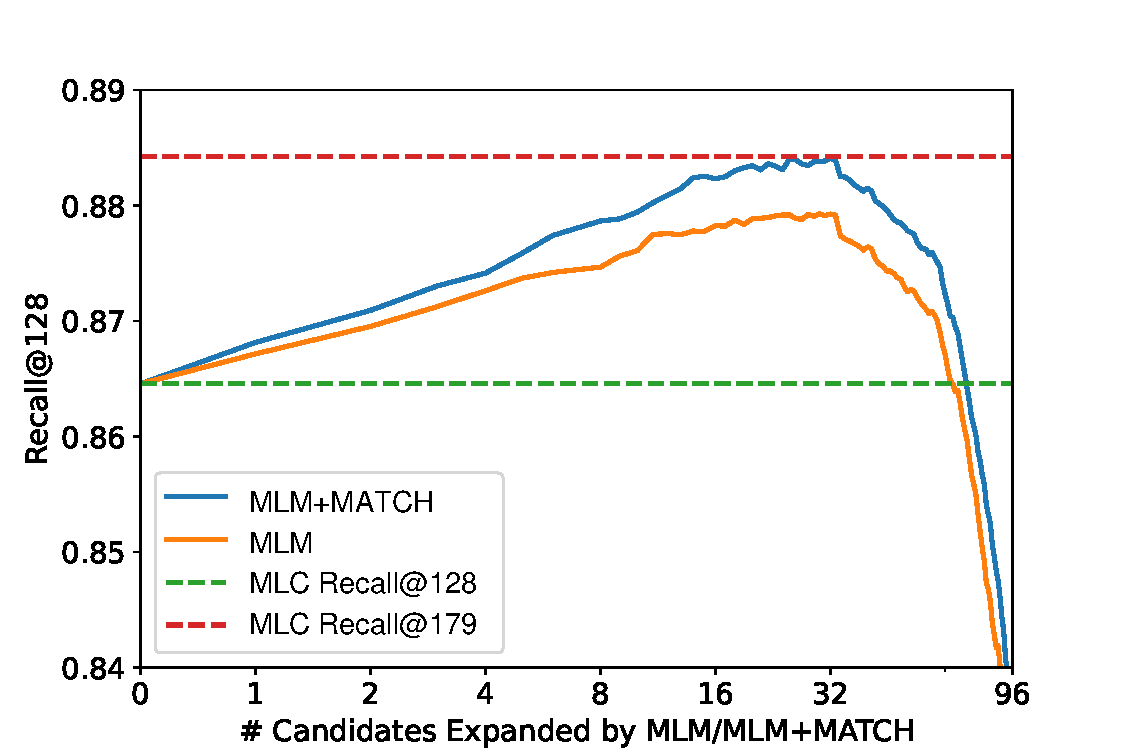
\includegraphics[width=\textwidth]{src/img/recall_ufet.pdf}
         \caption{Recall@$128$ on {\bf \textsc{UFET}} by including different number of expanded candidates. }
         \label{fig:c1}
     \end{subfigure}
     \vfill
     \begin{subfigure}[h]{0.45\textwidth}
         \centering
         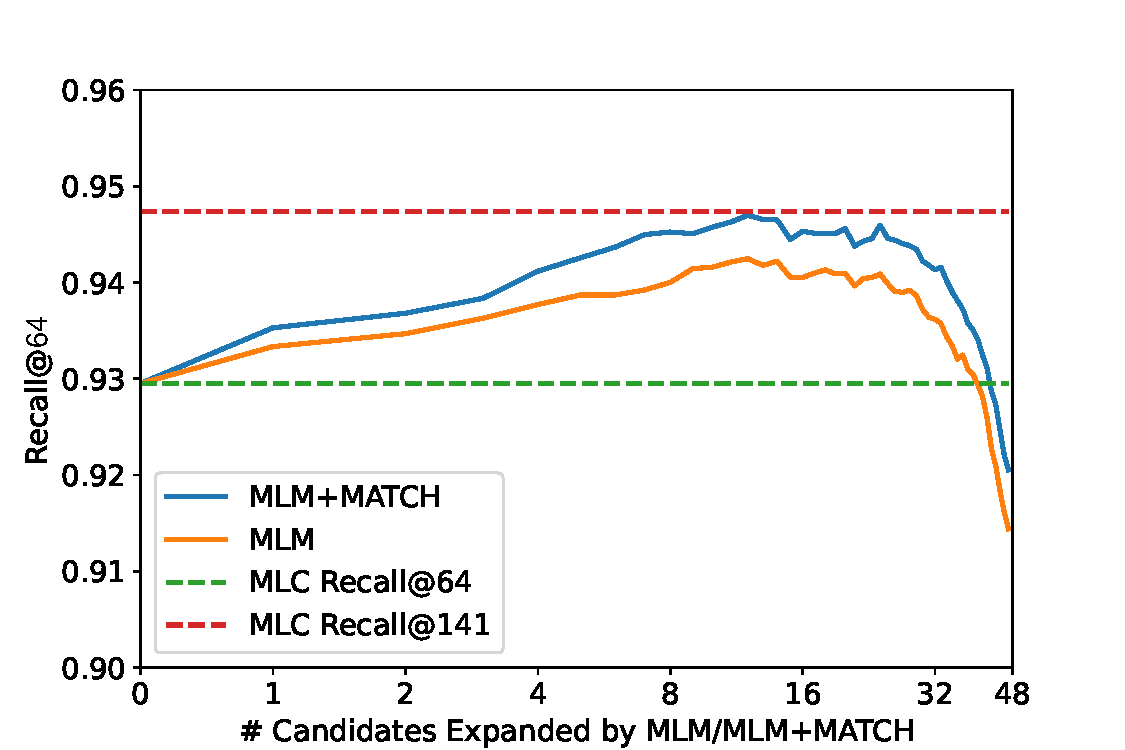
\includegraphics[width=\textwidth]{src/img/recall_cfet.pdf}
         \caption{Recall@$64$ on {\bf \textsc{CFET}} by including different number of expanded candidates.}
         \label{fig:c2}
     \end{subfigure}
\caption{Demonstration of the effect of expand stage. $x$-axis represents the number of candidates expanded by MLM/MLM+MATCH among these $128$ candidates. }
\label{fig:expand_improvement}
\end{figure}
\label{sec:exp_expand}
\subsection{Filter Stage and Final Results.}
\begin{table}[h!]
\centering
\scalebox{0.73}{
\renewcommand{\arraystretch}{1}
\begin{tabular}{cllll} \toprule
\multicolumn{2}{l}{\bf \textit{Base Models on UFET} }     & \bf \textsc{P}    & \bf \textsc{R}   & \bf \textsc{F1}  \\ \midrule
\multicolumn{5}{l}{\emph{MLC-like models}}        \\
\color{blue} \bf \texttt{B}& {\bf \textsc{Box4Types}}\cite{box4types}  & 52.8 & 38.8 & 44.8  \\
\color{blue}\bf \texttt{B}& {\bf \textsc{LDET}}$^\dagger$  \cite{onoe-durrett-2019-learning}          & 51.5 & 33.0 & 40.1 \\ 
\color{blue}\bf \texttt{B}& {\bf \textsc{MLMET}}$^\dagger$   {\cite{mlmet}}   & 53.6 & 45.3 & 49.1  \\
\color{blue}\bf \texttt{B}& {\bf \textsc{PL}}  \cite{ding2021prompt}   & 57.8 & 40.7 & 47.7 \\
\color{blue}\bf \texttt{B}& {\bf \textsc{DFET}}    \cite{dfet}      & 55.6 & 44.7 & 49.5 \\
\color{blue}\bf \texttt{B}& {\bf \textsc{MLC}} (reimplemented by us) & 46.5 & 34.9 & 39.9 \\ 
\color{red}\bf \texttt{R}& {\bf \textsc{MLC}} (reimplemented by us) & 42.2 & 44.9 & 43.5 \\ \hline 
\multicolumn{5}{l}{\emph{Seq2seq based models}}      \\
\color{blue}\bf \texttt{B} & {\bf \textsc{LRN} }  {\cite{liu-etal-2021-fine}}              & 54.5 & 38.9 & 45.4  \\\hline
\multicolumn{5}{l}{\emph{Filter models under our recall-expand-filter paradigm}}      \\
\color{blue}\bf \texttt{B} & {\bf \textsc{Vanilla CE}$_{128}$}   & 47.2 & 48.5 & 47.8 \\ 
\color{blue}\bf \texttt{B} & {\bf \textsc{\name-S$_{128}$}} (Ours)  & 53.2 & 48.3 & {\bf 50.6} \\ 
\color{blue}\bf \texttt{B} & {\bf \textsc{\name-S$_{128}$ w/o C2C}}   (Ours)   & 52.3 & 48.3 & 50.2 \\ 
\color{blue}\bf \texttt{B} & {\bf \textsc{\name-B$_{128}$}} (Ours)    & 49.9 & 50.0 & 49.9 \\ 
\color{blue}\bf \texttt{B} & {\bf \textsc{\name-B$_{128}$ w/o C2C}} (Ours)     & 49.9 & 48.2 & 49.0 \\ \hline
\color{red}\bf \texttt{R} & {\bf \textsc{Vanilla CE}$_{128}$}   & 49.6 & 49.0 & 49.3 \\ 
\color{red}\bf \texttt{R} & {\bf \textsc{\name-S$_{128}$}} (Ours)  & 53.3 & 47.3 & 50.1 \\ 
\color{red}\bf \texttt{R} & {\bf \textsc{\name-S$_{128}$ w/o C2C}}   (Ours)  & 53.2 & 46.6 & 49.7 \\ 
\color{red}\bf \texttt{R} & {\bf \textsc{\name-B$_{128}$}} (Ours)  & 52.5 & 47.9 & 50.1 \\ 
\color{red}\bf \texttt{R} & {\bf \textsc{\name-B$_{128}$ w/o C2C}} (Ours)     & 52.7 & 46.4 & 49.3 \\ \hline
\midrule
\multicolumn{2}{l}{\bf \textit{Large Models on UFET} }     & \bf \textsc{P}    & \bf \textsc{R}   & \bf \textsc{F1}  \\ \midrule
\multicolumn{5}{l}{\emph{MLC-like models}}        \\
\color{red}\bf \texttt{R} & {\bf \textsc{MLC}}  \cite{npcrf}               & 47.8 & 40.4 & 43.8  \\
\color{red}\bf \texttt{R} & {\bf \textsc{MLC-NPCRF}} \cite{npcrf}             & 48.7 & 45.5 & 47.0  \\
\color{red}\bf \texttt{R} & {\bf \textsc{MLC-GCN}} \cite{xiong-etal-2019-imposing}     & 51.2 & 41.0 & 45.5 \\
\color{blue}\bf \texttt{B} & {\bf \textsc{PL}}  \cite{ding2021prompt}       & 59.3 & 42.6 & 49.6  \\
\color{blue}\bf \texttt{B} & {\bf \textsc{PL-NPCRF}}  \cite{npcrf}  & 55.3 & 46.7 & {50.6}\\ \hline
\multicolumn{4}{l}{\emph{Cross-encoder based models and {\bf \textsc{\name}}s}}      \\
\color{red}\bf \texttt{R} & {\bf \textsc{LITE+L}}  \cite{lite}             & 48.7 & 45.8 & 47.2  \\
\color{teal}\bf \texttt{RM} & {\bf \textsc{LITE+NLI+L}} \cite{lite} & 52.4 & 48.9 & {50.6} \\ \hline
\multicolumn{4}{l}{\emph{Filter models under our recall-expand-filter paradigm}}   \\ 
\color{blue}\bf \texttt{B} & {\bf \textsc{Vanilla CE$_{128}$}}   & 50.3 & 49.6 & 49.9 \\ 
\color{blue}\bf \texttt{B} & {\bf \textsc{\name-S$_{128}$}}  (Ours)   & 52.5 & 49.1 & 50.8 \\ 
\color{blue}\bf \texttt{B} & {\bf \textsc{\name-S$_{128}$ w/o C2C}}   (Ours)   & 54.1 & 47.1 & 50.4 \\ 
\color{blue}\bf \texttt{B} & {\bf \textsc{\name-B$_{128}$}} (Ours)    & 54.0 & 48.6 & 51.2 \\ 
\color{blue}\bf \texttt{B} & {\bf \textsc{\name-B$_{128}$ w/o C2C}} (Ours)     & 52.8 & 48.3 & 50.4 \\ \hline
\color{red}\bf \texttt{R} & {\bf \textsc{Vanilla CE$_{128}$}}   & 54.5 & 49.3 & 51.8 \\ 
\color{red}\bf \texttt{R} & {\bf \textsc{\name-S$_{128}$}}  (Ours)   & 50.8 & 49.8  &  50.3 \\ 
\color{red}\bf \texttt{R} & {\bf \textsc{\name-S$_{128}$ w/o C2C}}   (Ours)   & 51.5 & 48.8 & 50.1 \\ 
\color{red}\bf \texttt{R} & {\bf \textsc{\name-B$_{128}$}} (Ours)    & 51.9 & 50.8 & 51.4 \\ 
\color{red}\bf \texttt{R} & {\bf \textsc{\name-B$_{128}$ w/o C2C}} (Ours)     & 51.6 & 51.6 & 51.6 \\ \hline
\color{teal}\bf \texttt{RM} & {\bf \textsc{\name-B$_{128}$ w/o C2C}} (Ours) & 56.3 & 48.5 & {\bf 52.1} \\ \hline
\midrule
\end{tabular}}
\caption{Macro-averaged UFET result. {\bf \textsc{LITE+L}} is LITE without NLI pretraining, {\bf \textsc{LITE+L+NLI}} is the full LITE model. Methods marked by $\dagger$ utilize either distantly supervised or augmented data for training. {\bf \textsc{\name-S$_{128}$}} denotes we use $128$ candidates recalled and expanded from the first two stages.}
\label{tab:ufet}
\end{table}
\begin{table}[t]
\centering
\scalebox{0.75}{
\renewcommand{\arraystretch}{1}
\begin{tabular}{cllll} \toprule
\multicolumn{2}{l}{\bf \textit{Models on CFET} }     & \bf \textsc{P}    & \bf \textsc{R}   & \bf \textsc{F1}  \\ \midrule
\multicolumn{5}{l}{\emph{MLC-like models}}        \\
\color{purple}\bf \texttt{N}& {\bf \textsc{MLC}} & 55.8 & 58.6 & 57.1 \\  
\color{purple}\bf \texttt{N}& {\bf \textsc{MLC-NPCRF}} \cite{npcrf}     & 57.0 & 60.5 & 58.7 \\ 
\color{purple}\bf \texttt{N}& {\bf \textsc{MLC-GCN}} \cite{xiong-etal-2019-imposing}   & 51.6 & 63.2 & 56.8 \\ 
\color{brown}\bf \texttt{C}& {\bf \textsc{MLC}} & 54.0 & 59.5 & 56.6 \\  
\color{brown}\bf \texttt{C}& {\bf \textsc{MLC-NPCRF}} \cite{npcrf}   & 54.0 & 61.6 & 57.3 \\  
\color{brown}\bf \texttt{C}& {\bf \textsc{MLC-GCN}} \cite{xiong-etal-2019-imposing} & 56.4 & 58.6 & 57.5 \\ \midrule 
\multicolumn{5}{l}{\emph{Filter models under our recall-expand-filter paradigm}}      \\
\color{purple}\bf \texttt{N} & {\bf \textsc{Vanilla CE}}   & 57.6 & 64.3 & 60.7 \\ 
\color{brown}\bf \texttt{C} & {\bf \textsc{Vanilla CE}}   & 54.0 & 63.3 & 58.3 \\  \hline
\color{purple}\bf \texttt{N} & {\bf \textsc{\name-S$_{64}$}} (Ours)  & 58.4 & 62.1 & 60.2 \\ 
\color{purple}\bf \texttt{N} & {\bf \textsc{\name-S$_{64}$ w/o C2C}}   (Ours)   & 59.1 & 61.5 & 60.3 \\ 
\color{purple}\bf \texttt{N} & {\bf \textsc{\name-B$_{64}$}} (Ours)    & 56.7 & 66.1 & 61.1 \\ 
\color{purple}\bf \texttt{N} & {\bf \textsc{\name-B$_{64}$ w/o C2C}} (Ours)     & 58.8 & 64.1 & 61.4 \\ \hline
\color{brown}\bf \texttt{C} & {\bf \textsc{\name-S$_{64}$}} (Ours)  & 55.5 & 62.6 & 58.8 \\ 
\color{brown}\bf \texttt{C} & {\bf \textsc{\name-S$_{64}$ w/o C2C}}   (Ours)   & 54.0 & 63.4 & 58.3 \\ 
\color{brown}\bf \texttt{C} & {\bf \textsc{\name-B$_{64}$}} (Ours)    & 55.0 & 63.5 & 59.0 \\ 
\color{brown}\bf \texttt{C} & {\bf \textsc{\name-B$_{64}$ w/o C2C}} (Ours)     & 57.3 & 61.3 & 59.3 \\ \hline
\midrule
\end{tabular}}
\caption{Macro-averaged CFET result.}
\label{tab:cfet}
\end{table}

In this section, we report the performance of {\bf \textsc{MCCE}} variants as the filter models and compare them with various strong baselines that we will introduce later. We also compare the inference speed of different models in this section. For filter models, we treat the number of candidates $K$ recalled and expanded by the first two stages as hyper-parameters, and tune it on the development set. We found the choice of PLM backbones has a non-negligible effect on the performance, and the PLM backbone of previous methods varies. Therefore for fairer comparisons to baselines, we conduct experiments of {\bf \textsc{\name}} using different backbone PLMs for our {\bf \textsc{\name}} models and report the results. For all {\bf \textsc{\name}} models, we use AdamW optimizer with a learning rate tuned between $5\times 10^{-6}$ and $2\times 10^{-5}$. The batch size we use is $4$ and we train the models for at most $50$ epochs with early stopping. {\bf \textsc{UFET}} also provides a large dataset obtained from distant supervision such as entity linking, we do not use it and only train and evaluate our models on human-labeled data.
\paragraph{Baselines}
The {\bf \textsc{MLC}} model we used for the recall stage and the cross-encoder ({\bf \textsc{CE}}) we introduced in Sec. \ref{sec:vanilla_ce} are natural baselines. We also compare our methods with recent PLM-based methods. {\bf \textsc{LDET} }\cite{onoe-durrett-2019-learning} is an MLC with Bert-base-uncased and ELMo \cite{elmo} trained on 727k examples automatically denoised from the distantly labeled UFET. {\bf \textsc{GCN} }\cite{xiong-etal-2019-imposing} uses GCN to model type correlations and obtain type embeddings. Types are scored by dot-product of mention and type embeddings. The original paper uses BiLSTM as the mention encoder and we use the results re-implemented by \citet{npcrf} using RoBERTa-large. {\bf \textsc{Box4Type} }\cite{box4types} uses Bert-large as the backbone and uses box embedding to encode mentions and types for training and inference. {\bf \textsc{LRN} }\cite{liu-etal-2021-fine} use Bert-base as the encoder and an LSTM decoder to generate types in a seq2seq manner. {\bf \textsc{MLMET} }\cite{mlmet} is a {\bf \textsc{MLC}} with Bert-base, but first pretrained by the distantly-labeled data augmented by masked word prediction, then finetuned and self-trained on the 2k human-annotated data. {\bf \textsc{PL}} \cite{ding2021prompt} uses prompt learning for entity typing. {\bf \textsc{DFET} }\cite{dfet} uses {\bf \textsc{PL}} as backbone and is a multi-round automatic denoising method for 2k labeled data. {\bf \textsc{LITE} }\cite{lite} is the previous SOTA system that formulates entity typing as textual inference. {\bf \textsc{LITE}} uses RoBERTa-large-MNLI as the backbone, and is a cross-encoder (introduced in Sec. \ref{sec:vanilla_ce}) with designed templates and a hierarchical loss. \citet{npcrf} proposes {\bf \textsc{NPCRF}} to enhance backbones such as {\bf \textsc{PL}} and {\bf \textsc{MLC}} by modeling type correlations, and reach performance comparable to {\bf \textsc{LITE}}.

\paragraph{Naming Conventions}
Let {\bf \textsc{\name-S}} be the {\bf \textsc{\name}} model that treats candidates as sub-tokens, and {\bf \textsc{\name-B}} be the model representing candidates as fixed-size blocks. The {\bf \textsc{\name}} model without {\bf \textsc{C2C}} attention (mentioned in Sec. \ref{sec:attn}) is denoted as {\bf \textsc{\name-B} w/o C2C}. For PLM backbones used in {\bf \textsc{UFET}}, we use {\color{blue} \bf \texttt{B}}, {\color{red} \bf \texttt{R}}, {\color{teal} \bf \texttt{RM}} to denote BERT-base-cased \cite{bert}, RoBERTa \cite{liu2019roberta}, and RoBERTa-MNLI \cite{liu2019roberta} respectively. For {\bf \textsc{CFET}}, we adopt two widely-used Chinese PLM, BERT-base-Chinese and NeZha-base-Chinese, and denote them as {\color{brown} \bf \texttt{C}} and {\color{purple} \bf \texttt{N}} respectively. 

\paragraph{UFET Results} We show the results of {\bf \textsc{UFET}} dataset in Table \ref{tab:ufet}. The results show that: (1) The recall-expand-filter paradigm is effective. Filter models outperform all baselines without the paradigm by a large margin. The vanilla CE under our paradigm reaches $51.8$ F1 compared to more complexed CE {\bf \textsc{LITE}} with $50.6$ F1 (2) {\bf \textsc{\name}} models reach SOTA performances. {\bf \textsc{\name-S$_{128}$}} with BERT-base performs best and reaches {\bf 50.6} F1 score, which is comparable to previous SOTA performance of large models such as {\bf \textsc{LITE+NLI+L}} and {\bf \textsc{PL+NPCRF}}. Among large models, {\bf \textsc{\name-B$_{128}$ w/o C2C}} also reaches SOTA performance with {\bf 52.1} F1 score. (3) {\bf \textsc{C2C}} attention is not necessary on large models, but is useful in base models. (4) Large models can utilize type semantics better. We found {\bf \textsc{\name-B}} outperforms {\bf \textsc{\name-S}} on large models, but underperforms {\bf \textsc{\name-S}} on base models. (5) Backbone PLM matters. We found the performance of {\bf \textsc{Vannila CE}} under our paradigm is largely affected by the PLM it used. It reaches $47.8$ F1 with BERT-base and $51.8$ F1 with RoBERTa-large. For {\bf \textsc{\name}} models, we found {\bf \textsc{\name}} performs better than {\bf \textsc{\name-B}} with BERT, and worse than {\bf \textsc{\name-B}} with RoBERTa. 

\begin{table*}[t]
\centering
\scalebox{0.9}{
\begin{tabular}{lllcc} \toprule
\bf \textsc{Model}  & \bf \textsc{\# FP} & \bf \textsc{Attn} & \bf \textsc{sents/sec} & \bf \textsc{F1} \\ \midrule
{\bf \textsc{MLC}} & \small{$1$}  & \small{$L_S^2D$} & 58.8 & 43.8\\
{\bf \textsc{LITE+NLI+L (CE)}}  & \small{$N$}  & \small{$L_S^2D$} & 0.02 & 50.6\\ \midrule \hline
\multicolumn{5}{l}{\emph{filter stage inference speed.}}  \\
{\bf \textsc{Vanilla CE$_{128}$}}  & \small{$128$}  & \small{$L_S^2D$} & 1.64 & 51.8 \\ 
{\bf \textsc{\name-S$_{128}$}}  & \small{$1$}  & \small{$(L_S+128)^2D$} & 60.8 & 50.1 \\ 
{\bf \textsc{\name-B$_{128}$}}  & \small{$1$}  & \small{$(L_S+128B)^2D$} & 22.3 & 51.4\\ 
{\bf \textsc{\name-B$_{128}$ w/o C2C}}  & \small{$1$}  & \small{$(L_S^2+256L_S B + 128 B^2)D$} & 25.2 & {\bf 52.1}\\ \bottomrule
\end{tabular}}
\caption{Inference speed comparison of models. {\bf \textsc{\# FP}} means the number of PLM forward passes required by a single inference. {\bf \textsc{ATTN}} column lists the theoretical attention complexity.  We also report the practical inference speed {\bf \textsc{sents/sec}} and the {\bf \textsc{F1}} scores on {\bf \textsc{UFET}} with RoBERTa-large architecture.}
\label{tab:speed}
\end{table*}

\begin{table}[t]
\centering
\scalebox{0.85}{
\renewcommand{\arraystretch}{1}
\begin{tabular}{cllll} \toprule
\multicolumn{2}{l}{\bf \textit{Models} }     & \bf \textsc{P}    & \bf \textsc{R}   & \bf \textsc{F1}  \\ \midrule
\multicolumn{5}{l}{\emph{coarse (9 types) Open Entity}}        \\ \hline
\color{red}\bf \texttt{R} & {\bf \textsc{MLC}}   & 76.8 & 78.5 & 77.6 \\ 
\color{red}\bf \texttt{R} & {\bf \textsc{Vanilla CE$_{9}$}}   & 82.3 & 81.0 & 81.6 \\ 
\color{red}\bf \texttt{R} & {\bf \textsc{\name-S$_{9}$}}   & 77.0 & 87.7 & 82.0 \\ 
\color{red}\bf \texttt{R} & {\bf \textsc{\name-B$_{9}$ w/o C2C}}   & 77.2 & 85.4 & 81.1 \\ \hline
\multicolumn{5}{l}{\emph{fine (130 types)}}        \\ \hline
\color{red}\bf \texttt{R} & {\bf \textsc{MLC}}   & 70.4 & 63.7 & 66.9  \\ 
\color{red}\bf \texttt{R} & {\bf \textsc{Vanilla CE}$_{130}$}   & 67.9 & 66.4 & 67.1 \\ 
\color{red}\bf \texttt{R} & {\bf \textsc{\name-S$_{130}$}}   & 65.8 & 71.8 & 68.7 \\ 
\color{red}\bf \texttt{R} & {\bf \textsc{\name-B$_{130}$ w/o C2C}}   & 64.1 & 70.5 & 67.1 \\ \hline
\midrule
\end{tabular}}
\caption{Micro-averaged results on UFET fine and coarse.}
\label{tab:ufet-coarse-fine}
\end{table}

\paragraph{CFET Results} We conduct experiments on {\bf \textsc{CFET}} and compare {\bf \textsc{\name}} models with several strong baselines:  {\bf \textsc{NPCRF}} and {\bf \textsc{GCN}} with MLC-like architecture, and {\bf \textsc{Vanilla CE}} under out paradigm which is proved to be better than {\bf \textsc{LITE}} on {\bf \textsc{UFET}}. The results are shown in Table \ref{tab:cfet}. Similar to results in {\bf \textsc{UFET}}, filter models under our paradigm significantly outperform MLC-like baselines, $+2.0$ F1 for Nezha-base and $+1.8$ F1 for BERT-base-Chinese. In {\bf \textsc{CFET}}, {\bf \textsc{\name}-B} is significantly better than {\bf \textsc{\name}-S}, on both Nezha-base and BERT-base-Chinese, indicating the importance of type semantics in Chinese language. We also find that {\bf \textsc{\name} w/o C2C} is generally better than  {\bf \textsc{\name} w/ C2C}, it is possibly because the C2C attention distracts the candidates from attending to mention and contexts.
\paragraph{Speed Comparison} Table \ref{tab:speed} shows the theoretical inference complexity (number of PLM forward passes, and attention complexity), and practical inference speed (number of sentences inferred per second) of different models. We conduct the speed test using NVIDIA TITAN RTX for all models, and the inference batch size is 4.
At the filter stage, the inference speed of {\bf \textsc{\name-S}} is on par with {\bf \textsc{MLC}} (even slightly faster because we don't need to score all types), and is about 40 times faster than {\bf \textsc{Vannila CE}} and thousands of times faster than {\bf \textsc{LITE}}. {\bf \textsc{\name-B w/o C2C}} is not significantly faster than {\bf \textsc{\name-B}} as expected. It's possibly because the computation related to the block attention is not fully optimized by existing deep learning frameworks. The speed advantage of {\bf \textsc{\name-B w/o C2C}} over {\bf \textsc{\name-B}} will be greater with more candidates.


\subsection{Fine-grained and Coarse-grained Entity Typing}
We also conduct experiments on Fine-grained (130-class) and Coarse-grained (9-class, also known as ``Open Entity'') entity typing, and the results are shown in Table \ref{tab:ufet-coarse-fine}. As the type candidate set is much smaller in these settings, we skip the recall and expand stages and directly run the filter models and compare them to baselines. Results show that both {\bf \textsc{\name}-S} and {\bf \textsc{\name}-B} are still better than {\bf \textsc{MLC}} and {\bf \textsc{Vanilla CE}}, and {\bf \textsc{\name}-S} is better than {\bf \textsc{\name}-B} on coarser-grained cases possibly because the coarser-grained types are simpler in surface-forms and {\bf \textsc{\name}-S} will not lose many type semantics.





\label{sec:analysis}
We now study \method{} from a graph convolution perspective. We demonstrate that \method{} corresponds to a fixed filter on the graph spectral domain. 
In addition, we show that adding self-loops to the original graph, i.e. the renormalization trick \citep{gcn}, effectively shrinks the underlying graph spectrum.
On this scaled domain, \method{} acts as a low-pass filter that produces smooth features over the graph. As a result, nearby nodes tend to share similar representations and consequently predictions.


\subsection{Preliminaries on Graph Convolutions}
Analogous to the Euclidean domain, graph Fourier analysis relies on the spectral decomposition of graph Laplacians. The graph Laplacian $\boldsymbol{\Delta} = \rmD - \rmA$ (as well as its normalized version $\boldsymbol{\Delta}_{\text{sym}} = \rmD^{-1/2}\boldsymbol{\Delta} \rmD^{-1/2}$) is a symmetric positive semidefinite matrix with eigendecomposition $\boldsymbol{\Delta} = \rmU \boldsymbol{\Lambda} \rmU^{\top}$, where $\rmU \in \mathbb{R}^{n \times n}$ comprises orthonormal eigenvectors and $\boldsymbol{\Lambda} = \text{diag}(\lambda_1, \dots, \lambda_n)$ is a diagonal matrix of eigenvalues. The eigendecomposition of the Laplacian allows us to define the Fourier transform equivalent on the graph domain, where eigenvectors denote Fourier modes and eigenvalues denote frequencies of the graph. In this regard, let $\rvx \in \mathbb{R}^n$ be a signal defined on the vertices of the graph. We define the graph Fourier transform of $\rvx$ as $\hat{\rvx} = \rmU^{\top}\rvx$, with inverse operation given by $\rvx = \rmU \hat{\rvx}$.
Thus, the graph convolution operation between signal $\rvx$ and filter $\rvg$ is
\begin{equation} \label{eq:spectral_conv_definition}
    \rvg * \rvx = \rmU \left( (\rmU^\top \rvg) \odot (\rmU^\top \rvx) \right) = \rmU \hat{\rmG} \rmU^\top \rvx,
\end{equation}
where $\hat{\rmG} = \text{diag}\left(\hat{g}_1, \dots, \hat{g}_n\right)$ denotes a diagonal matrix in which the diagonal corresponds to spectral filter coefficients. 

Graph convolutions can be approximated by $k$-th order polynomials of Laplacians
\begin{equation}
\label{eq:polynomial approximation}
    \rmU\hat{\rmG}\rmU^\top\rvx \approx \sum_{i=0}^{k} \theta_i \boldsymbol{\Delta}^i \rvx = \rmU \left( \sum_{i=0}^{k} \theta_i \boldsymbol{\Lambda}^i \right) \rmU^\top \rvx,
\end{equation}
where $\theta_i$ denotes coefficients. In this case, filter coefficients correspond to polynomials of the Laplacian eigenvalues, i.e., $\hat{\rmG} = \sum_i \theta_i \boldsymbol{\Lambda}^i$ or equivalently $\hat{g}(\lambda_j) = \sum_i \theta_i \lambda_j^i$. 


Graph Convolutional Networks (GCNs) \cite{gcn} employ an affine approximation ($k=1$) of \autoref{eq:polynomial approximation} with coefficients $\theta_0=2\theta$ and $\theta_1=-\theta$ from which we attain the basic GCN convolution operation
\begin{equation} \label{eq:first-order-cheby}
    \rvg * \rvx = \theta (\rmI + \rmD^{-1/2} \rmA \rmD^{-1/2}) \rvx.
\end{equation}

In their final design, \citet{gcn} replace the matrix $\rmI + \rmD^{-1/2} \rmA \rmD^{-1/2}$ by a normalized version $\tilde{\rmD}^{-1/2} \tilde{\rmA} \tilde{\rmD}^{-1/2}$ where $\tilde{\rmA} = \rmA + \rmI$ and consequently $\tilde{\rmD} = \rmD + \rmI$, dubbed the \textit{renormalization trick}. Finally, by generalizing the convolution to work with multiple filters in a $d$-channel input and layering the model with nonlinear activation functions between each layer, we have the GCN propagation rule as defined in \autoref{eq:gcn_propagation}.

\begin{figure*}[tb] 
\centering
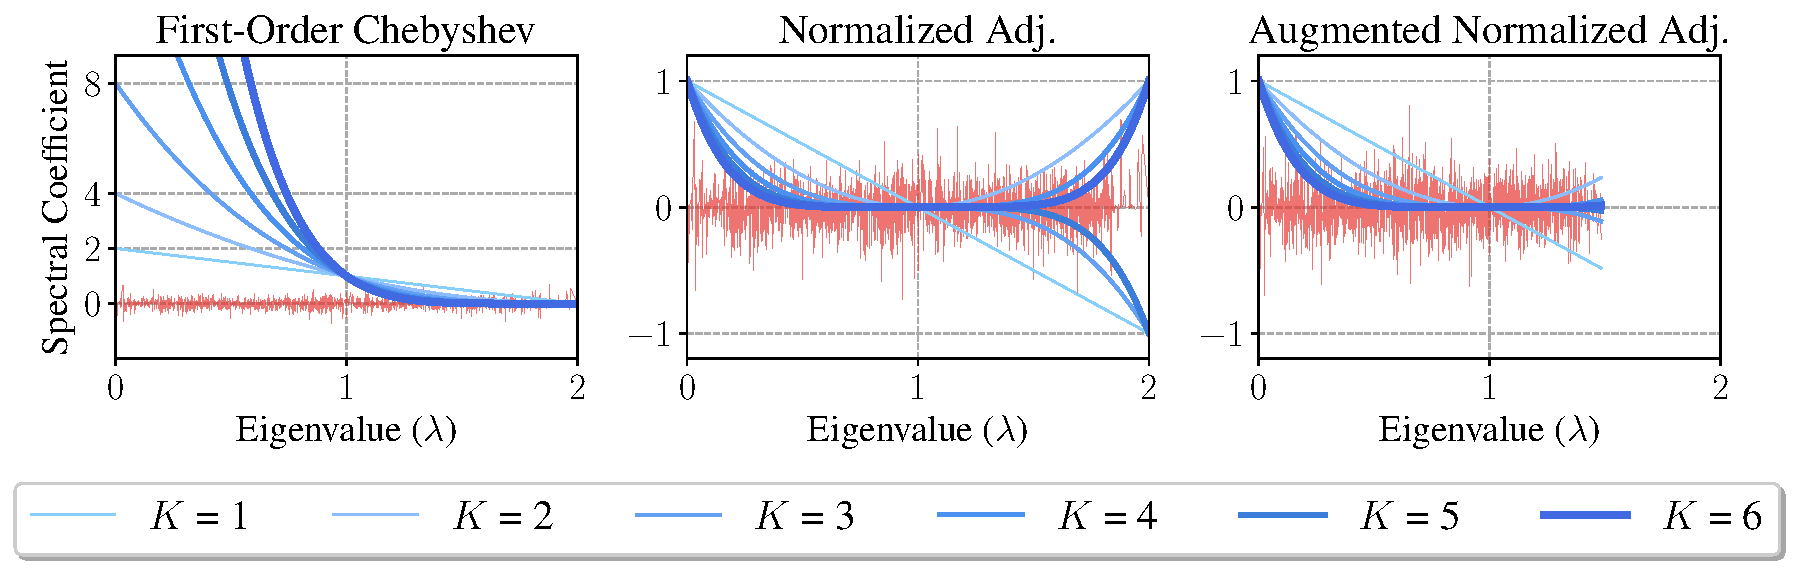
\includegraphics[width=.8\linewidth]{figures/s_filters_new2.pdf}
\caption{Feature ({\color{myred}red}) and filters ({\color{myblue}blue}) spectral coefficients for different propagation matrices on Cora dataset ($3$rd feature).}
\label{fig:s_filters}
\end{figure*}

\subsection{\method{} and Low-Pass Filtering}
The initial first-order Chebyshev filter derived in GCNs corresponds to the propagation matrix $\rmS_{\text{1-order}} = \rmI + \rmD^{-1/2} \rmA \rmD^{-1/2}$ (see \autoref{eq:first-order-cheby}). Since the normalized Laplacian is $\boldsymbol{\Delta}_{\text{sym}} = \rmI - \rmD^{-1/2} \rmA \rmD^{-1/2}$, then $\rmS_{\text{1-order}} = 2\rmI - \boldsymbol{\Delta}_{\text{sym}}$. Therefore, feature propagation with $\rmS_{\text{1-order}}^K$ implies filter coefficients $\hat{g}_i = \hat{g}(\lambda_i) = (2 - \lambda_i)^K$, where $\lambda_i$ denotes the eigenvalues of $\boldsymbol{\Delta}_{\text{sym}}$. \autoref{fig:s_filters} illustrates the filtering operation related to $\rmS_{\text{1-order}}$ for a varying number of propagation steps $K \in \{1,\dots, 6\}$. As one may observe, high powers of $\rmS_{\text{1-order}}$ lead to exploding filter coefficients and undesirably over-amplify signals at frequencies $\lambda_i < 1$.


To tackle potential numerical issues associated with the first-order Chebyshev filter, \citet{gcn} propose the \textit{renormalization trick}. Basically, it consists of replacing $\rmS_{\text{1-order}}$ by the normalized adjacency matrix after adding self-loops for all nodes. We call the resulting propagation matrix the augmented normalized adjacency matrix $\tilde{\rmS}_{\text{adj}} = \tilde{\rmD}^{-1/2}\tilde{\rmA}\tilde{\rmD}^{-1/2}$, where $\tilde{\rmA}=\rmA+\rmI$ and $\tilde{\rmD}=\rmD+\rmI$. Correspondingly, we define the augmented normalized Laplacian $\tilde{\boldsymbol{\Delta}}_{\text{sym}} = \rmI -  \tilde{\rmD}^{-1/2}\tilde{\rmA}\tilde{\rmD}^{-1/2}$. Thus, we can describe the spectral filters associated with $\tilde{\rmS}_{\text{adj}}$ as a polynomial of the eigenvalues of the underlying Laplacian, i.e.,  $\hat{g}(\tilde{\lambda}_i) = (1 - \tilde{\lambda}_i)^K$, where $\tilde{\lambda}_i$ are eigenvalues of $\tilde{\boldsymbol{\Delta}}_{\text{sym}}$.


We now analyze the spectrum of $\tilde{\boldsymbol{\Delta}}_{\text{sym}}$ and show that adding self-loops to graphs shrinks the spectrum (eigenvalues) of the corresponding normalized Laplacian.

\begin{theorem}\label{thm:Lapla_eig_shrink} Let $\rmA$ be the adjacency matrix of an undirected, weighted, simple graph $\mathcal{G}$ without isolated nodes and with corresponding degree matrix $\rmD$. Let $\tilde{\rmA} = \rmA + \gamma \rmI$, such that $\gamma > 0$, be the augmented adjacency matrix with corresponding degree matrix $\tilde{\rmD}$. Also, let $\lambda_1$ and $\lambda_n$ denote the smallest and largest eigenvalues of $\boldsymbol{\Delta}_{\text{sym}}=\rmI -  \rmD^{-1/2}\rmA\rmD^{-1/2}$; similarly, let $\tilde{\lambda}_1$ and $\tilde{\lambda}_n$ be the smallest and largest eigenvalues of $\tilde{\boldsymbol{\Delta}}_{\text{sym}}=\rmI -  \tilde{\rmD}^{-1/2}\tilde{\rmA}\tilde{\rmD}^{-1/2}$. We have that
\begin{equation}
0 = \lambda_1 = \tilde{\lambda}_1 < \tilde{\lambda}_n < \lambda_n. \label{eq:corollary_aug_laplacian}
\end{equation}
\end{theorem}
%
\autoref{thm:Lapla_eig_shrink} shows that the largest eigenvalue of the normalized graph Laplacian becomes smaller after adding self-loops $\gamma > 0$ (see supplementary materials for the proof).

\autoref{fig:s_filters} depicts the filtering operations associated with the normalized adjacency $\rmS_{\text{adj}} = \rmD^{-1/2}\rmA\rmD^{-1/2}$ and its augmented variant $\tilde{\rmS}_{\text{adj}} =  \tilde{\rmD}^{-1/2}\tilde{\rmA}\tilde{\rmD}^{-1/2}$ on the Cora dataset~\citep{sen2008collective}. Feature propagation with $\rmS_{\text{adj}}$ corresponds to filters $g(\lambda_i) = (1-\lambda_i)^K$ in the spectral range $[0, 2]$; therefore odd powers of $\rmS_{\text{adj}}$ yield negative filter coefficients at frequencies $\lambda_i > 1$. By adding self-loops ($\tilde{\rmS}_{\text{adj}}$), the largest eigenvalue shrinks from $2$ to approximately $1.5$ and then eliminates the effect of negative coefficients. Moreover, this scaled spectrum allows the filter defined by taking powers $K>1$ of $\tilde{\rmS}_{\text{adj}}$ to act as a low-pass-type filters. In supplementary material, we empirically evaluate different choices for the propagation matrix.
\section{Related Work}
While writing this paper, we noticed that a paper \cite{Du2022LearningTS} that has similar ideas to our work was submitted to the arXiv. They propose a two-stage paradigm for selecting from multiple questions. They also propose a network similar to our {\bf \textsc{\name-B}} to select from multiple options in parallel. We summarize the differences between their work and ours as follows: (1) Different in paradigm. We have an expand stage to further improve the quality of recalled candidates (2) Different in models. {\bf \textsc{\name-S}} and {\bf \textsc{\name-B}} are both different from theirs in both input format and scoring. We additionally propose to discard the C2C attention and study the effect of removing different parts of attention. (3) We focus more on entity typing and conduct extensive experiments covering two languages and three settings (ultra-fine-grained, fine-grained, and coarse-grained). We analyze the effect of using different PLM backbones for a fairer and more comprehensive comparison.
The paradigm of our work is also inspired by works in entity linking and information retrieval. \citet{wu2019zero} uses a retrieval and rerank paradigm for entity linking, they first generate entity candidates using a bi-encoder and rerank them using a vanilla cross-encoder. Our paradigm with an additional expand stage and our proposed {\bf \textsc{\name}} models are also potentially useful for entity linking. We leave it for future work. \citet{halter} represents the query document and candidate documents as vectors and proposed to use a transformer to rerank all candidate documents in parallel for passage retrieval. Compared to them, we tackle entity typing and preserve all information of mention and context rather than represent them as a single vector, the paradigm, model architecture, and training objective are also different.





\section{Conclusion}
\label{sec_conclusions}

Our work consists of two studies that quantitatively and qualitatively investigate the influence of a CI service (e.g., \textsc{TravisCI}), and CI as a practice, on the time-to-delivery of merged PRs, respectively. In our quantitative study, we analyze 162,653 PRs of 87 GitHub projects to understand the factors that influence (and improve) the delivery time of merged PRs. In our qualitative study, we analyze 450 survey responses from participants of 73 projects (out of the initial 87 projects). We investigate the perceived influence of CI on the delivery time of merged PRs. We also study the perceived influence of CI on the code review and release processes.

As a key takeaway, our studies demonstrate that the adoption of \textsc{TravisCI}
will not necessarily deliver or merge PRs more quickly. Instead, the pivotal benefit of a CI service is to improve the mechanisms by which contributions to projects are processed (e.g., facilitating decisions on PR submissions), without compromising the quality of the project or overloading developers. The automation provided by CI and the boost in developers' confidence are key aspects of using CI. For instance, CI may help the process of sorting which PRs are worth reviewing (e.g., PRs with green builds).
Furthermore, open-source projects wishing to attract and retain external contributors should consider the use of CI in their pipeline, since CI is perceived to lower the contribution barrier while making contributors feel more confident and engaged in the project.

\section*{Acknowledgments}
\label{sec_Acknowledgments}

This work is partially supported by INES (\url{www.ines.org.br}), CNPq grants 465614/2014-0 and 425211/2018-5, CAPES grant 88887.136410/2017-00, FACEPE grants APQ-0399-1.03/17, and PRONEX APQ/0388-1.03/14.

\section*{Data Availability}
For replication purposes, we publicize our datasets and results to the interested researcher: \url{https://prdeliverydelay.github.io/#datasets}

\section*{Declarations}

\textbf{Conflict of interests}. The authors declare that they have no conflict of interest.

% Entries for the entire Anthology, followed by custom entries
\bibliography{main}
\bibliographystyle{acl_natbib}

% \appendix
% \section{Example Appendix}
% \label{sec:appendix}
\end{document}
